In this chapter, we aim to validate our analysis of the trade-offs involved in query processing state placement decisions,
and to evaluate the effectiveness of our design and prototype implementation in providing an effective mechanism to applications
for navigating these trade-offs.

This evaluation consists of two parts.
The first part (\S\ref{sec:eval_1}) is based on the case study of a read-heavy web application, presented in Section~\ref{sec:lobsters}.
It focused on the placement of a materialized view,
and examines two placement options: in the data center, close to the corpus, or at the edge close to the clients.
The aim of the first part is to answer the following questions:

\begin{itemize}

  \item What is the overhead of materializing state in Proteus, directly over the data storage tier?
  (Section~\ref{sec:eval_query_processing_perf})

  \item What improvements in query processing performance can be achieved by placing materialized state close to clients?
  (Section~\ref{sec:eval_query_processing_perf})

  \item What are the penalties in freshness incurred when placing materialized state away from the data storage tier
  (Section~\ref{sec:eval_freshness})?
  How is freshness affected by load (\S\ref{sec:eval_freshness_throughput}) and round-trip time between
  sites (\S\ref{sec:eval_freshness_rtt})?

  \item What additional data transfer costs result from materialized state placed close to clients receiving updates?
  (Section~\ref{sec:eval_data_transfer})

\end{itemize}

The second part (\S\ref{sec:eval_2}) of the evaluation is based on the case study of federated query processing on a multi-cloud
corpus, presented in Section~\ref{sec:zenko}.
In this part we examine three partitioning and placement configurations for a multi-cloud secondary index.
We compare the three configurations under different types of workloads, and evaluate three metrics:
query processing performance, freshness and data transfer costs.

The aim of the second part is to (1) demonstrate the expressiveness of the QPU approach,
by deploying and comparing three query engine configurations across 3 data centers without any changes to the client application and the storage tier,
and (2) validate that by controlling the configuration of QPU-based query engines,
applications can navigate the trade-offs of geo-distributed query processing and optimize for different criteria according to their needs.


\section{Placing materialized views at the edge}
\label{sec:eval_1}

\subsection{Experimental scenario}
\label{sec:eval_scenario}

The evaluation in this section is based on the case study presented in Section~\ref{sec:lobsters},
which describes the Lobsters \cite{lobste:rs} web application.
We choose this application for the following reasons:
\begin{itemize}
\item It is characterized by a query-heavy workload that requires the materialization of derived state,
and derived state is updated by a stream of small updates.
This make Lobsters suitable for evaluating the efficacy of our design and prototype implementation in
navigating the trade-offs of query processing state placement,
by examining the effect of different placement schemes in query performance and query result freshness.

\item It open-source \cite{lobsters:source},
allowing us to examine the application's interaction with the database in which it stores its state,
and statistics about the application's data usage patterns are available \cite{lobste:stats}.

\item It resembles a class of popular large-scale web applications, such as Reddit and Hacker News.
\end{itemize}

\bigskip
\noindent
In Lobsters, users post, comment, and vote on ``stories''.
Each story is associated with a ``hotness'' value that indicates how popular it is.
Stories are ranked by hotness;
the stories with the highest hotness value appear on the front page.
The hotness value of a story depends on parameters such as the number of votes for the story,
the number of comments, and the hotness of those comments.
Various operations, such as voting or commenting on a story, modify the hotness value.
Computing the hotness value when it is queried would impose a prohibitive delay on queries
% It is prohibitively expensive \cite{gjengset:noria} to compute the hotness value of stories during queries.
In particular, serving the Lobsters' front page requires computing the hotness of every story in order to rank them.
That is why the Lobsters application adds an additional column to the $stories$ table which stores a pre-computed
hotness value for each story.
The application updates the value of the hotness column when operations are performed,
such as upvoting or downvoting a story, or adding a comment to a story.

For this evaluation, we consider a version of the Lobsters application, that consists of two operations:
voting for stories, and requesting the front page.
We choose this simplified model of the application because it gives us better control over the properties of the workload
for the purposes of this evaluation,
while also capturing the aspects of the Lobsters application that make is suitable for this evaluation.

In particular, we consider the following database schema:

\begin{lstlisting}[caption={Simplified Lobsters schema used in this evaluation.}]
TABLE users (id bigint, username varchar(50))
TABLE stories (id bigint, user_id bigint, title varchar(150), description mediumtext, short_id varchar(6));
TABLE votes (id bigint, user_id bigint, story_id bigint, vote tinyint);
\end{lstlisting}

The front page is a listing of the 25 most highly ranked stories, including their title, author, and vote count.
In the statistics provided by the Lobsters administrators, the front page operation constitutes 30.1\% of client requests,
and voting on stories constitutes 0.5\% of client requests.
The workload used for this evaluation consists of 95\% front page operations, and 5\% voting operations, unless otherwise specified.

\begin{table}[H]
\centering
\begin{tabular}{|c||c|c|c|c|c|c|}
\hline
Number of votes & [0-10) & [10-20) & [20-30) & [30-40) & [40-50) & [50-60) \\
\hline
\% of stories & 41.1 & 40.3 & 11.3 & 4.2 & 1.6 & 1.3 \\
\hline
\end{tabular}
\caption{Distribution of votes to stories in the Lobsters statistics \cite{lobste:stats}.}
\label{tab:votes_per_story}
\end{table}

According to the available data \cite{lobste:stats}, most stories (81.4\%) receive between 0 and 20 votes,
while about 7\% receive 30 votes or more.
Our experiments show that when votes follow this distribution,
very few votes are performed on the stories on the front page to have meaningful impact on query result freshness.
To address that, we use a more skewed distribution:
We configure 60\% of votes to target the 25 stories in the front page, and 40\% to follow the distribution shown in Table~\ref{tab:votes_per_story}.

\begin{figure}[H]
  \centering
    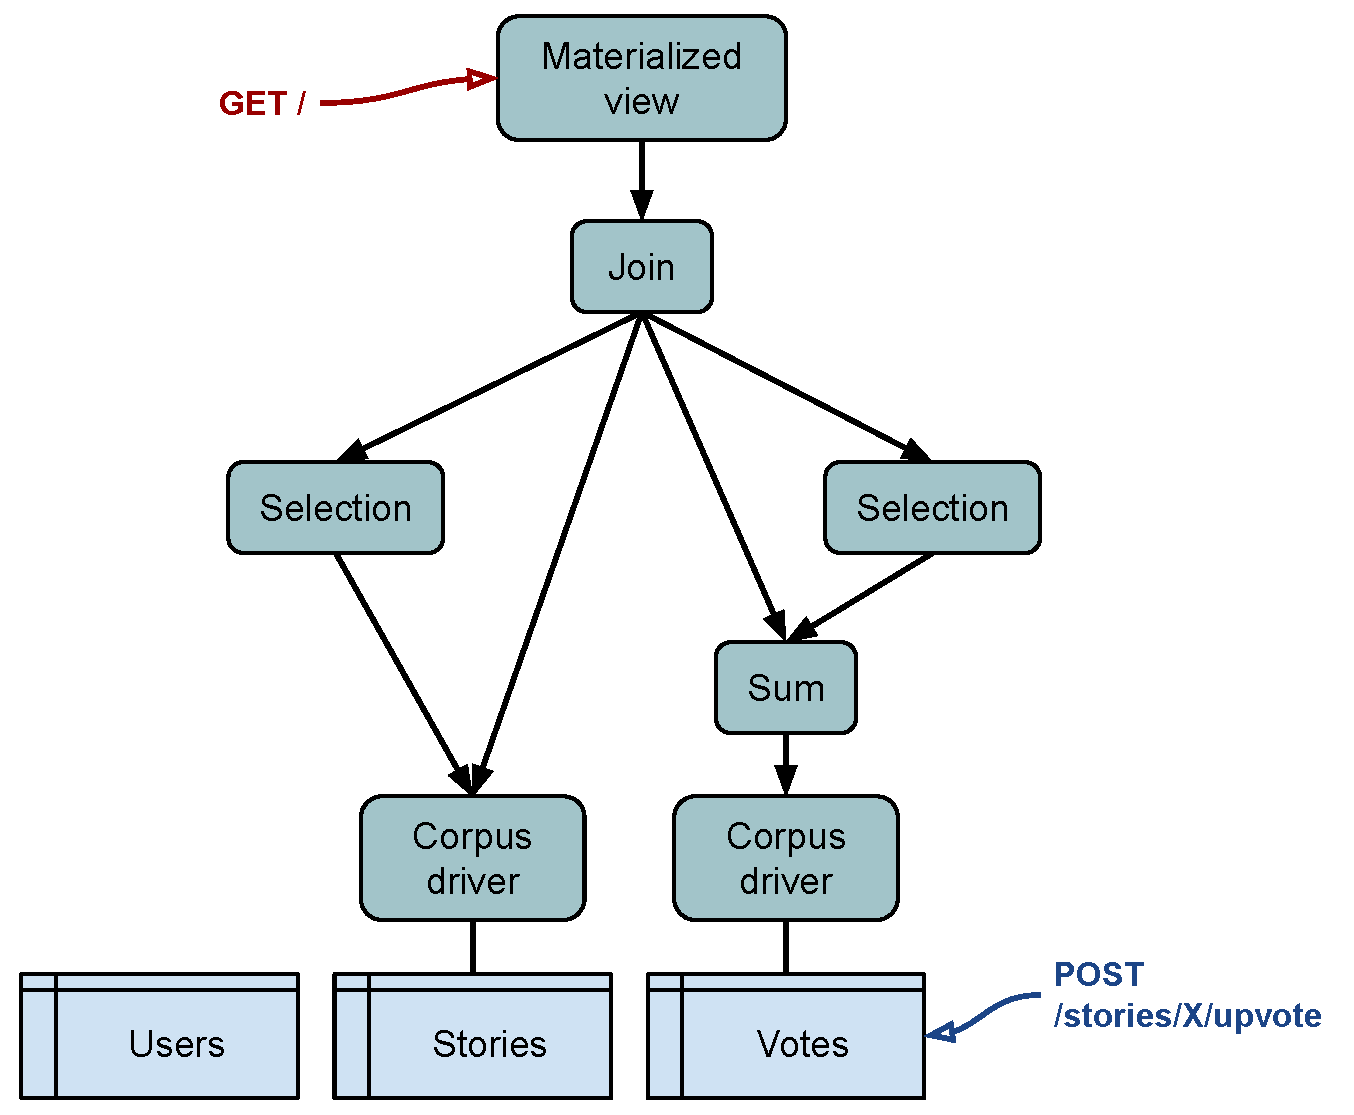
\includegraphics[scale=0.5]{./figures/evaluation/lobsters_architecture_eval.pdf}
  \caption{QPU graph used for this evaluation. The Materialized view QPU computes the vote count for each story,
  and joins it with the corresponding record from the $stories$ stable.
  The ``GET /'' request indicates the front page operation, and the ``POST /stories/X/upvote'' request indicates the operation of voting up story X.}
  \label{fig:eval_lobsters_qpu_arch}
\end{figure}

\bigskip
\noindent
The evaluation uses the QPU graph depicted in Figure~\ref{fig:eval_lobsters_qpu_arch} to maintain a materialized view that
pre-computes the vote count of each count and joins it to the corresponding record of the $stories$ table.
The materialized view is defined by the following query:

\begin{lstlisting}[caption={Definition of the materialized view maintained by the QPU graph shown in Figure~\ref{fig:eval_lobsters_qpu_arch}.}]
SELECT id, author_id, title, url, vote_count
FROM stories
JOIN (
  SELECT story_id, SUM(vote) as vote_count
  FROM votes
  GROUP BY story_id
) view
ON stories.id = view.story_id
\end{lstlisting}

This simplifies both the vote and front page operations compared to the baseline Lobsters implementation:
the vote operation does not need to explicitly update the vote count of the given story, as this
is performed by the QPU graph,
and the front page operation can be served from the materialized view.

In the actual QPU graph deployed for the experiments, each Selection QPU is merged with its downstream connection,
in a single unit that performs both functionalities.
In addition, the Materialized View is merged with the Join QPU.

The Materialized view QPU implementation used in these experiments stores its state in a MariaDB instance.
This is a separate instance from the one that is used the Lobsters database.
It is deployed alongside and only accessible by the Materialized view QPU.
The choice of using the same database both as the baseline and for storing the materialized view is aimed at eliminating
the effect of the database performance from the evaluation results,
providing a comparison that isolates the effects of placement.

Finally, we create an index on the table that implements the materialized view in order to support efficient retrieval of
the stories with the highest vote count.

\bigskip
\noindent
We consider a system topology consisting of two geographically distant sites:
The Lobsters application is deployed on one site, called server site,
and clients are located on another site, called client site.
Round-trip time between these two sites is 80 ms.
This corresponds to a scenario in which the Lobsters web application is deployed in a data centers in North America,
and clients are located in Europe \cite{pbailis:hats}, or vice versa.

Our experiments  make use of the ability to place QPUs strategically in the system topology.
We use two placement schemes:
One in which the Materialized view QPU is placed at the server site, and one in which it is placed at
the client site.
We evaluate the effects and trade-offs of materialized view placement by comparing these two placement schemes.


\subsection{Experimental Setup}
\label{sec:eval_setup}

While the actual Lobsters Ruby-on-Rails application is open-source,
we use a simplified version of it in order to isolate its interaction with the database.
We implement an adapter that translates front page and vote requests to the queries that the real
Lobsters application would issue, and issues those queries either to the Lobsters database (MariaDB),
or MariaDB and Proteus, depending on the experiment configuration.
This allows us to isolate the interaction between the application and the database, which is the focus of this work,
and remove other tasks that the Lobsters application performs, which quickly become a bottleneck.

We implement this adapter as a server-side component:
it is deployed along with the database on the server site, and plays the role of a simplified web server:
It exposes a gRPC endpoint, similar to the QPU gRPC server, and clients issue operations to it as RPC requests.
We choose this configuration because our initial experiments showed that issuing a large number of concurrent transactions
to MariaDB under a 80 ms client-server round-trip time results in errors both in the database,
and the Go MySQL library.

\bigskip
\noindent
\textbf{Workload generation.}
We implement a workload generator \cite{lobsters:bench} that is responsible for issuing
requests to the Lobsters adapter.
The workload generator uses an open-loop model \cite{schroeder:cautionarytale}:
it creates requests based on a target load (requests submitted per second) value;
each request is executed by a separate thread (creating and destroying threads are low-cost operations because threads are
implemented as Goroutines).

In addition, the workload generator measures throughput and response time.
We define response time as the delay that a client application experiences between issuing a request and receiving the
corresponding response.
To capture the variance of response time, we use a histogram data structure provided by the Go implementation of gRPC \cite{grpcgo:histogram}
that accumulates values in a histogram with exponentially increasing bucket sizes, in order to compute response time percentiles.

Our experiments show that while the open-loop design is effective at generating the target load
both under low and high client-server round-trip times (in closed-loop designs, high round-trip times result in lower offered load),
it results in a positive feedback loop effect above a certain load threshold:
When the system starts not being able to handle the offered load, response time increases.
However, the workload generator keeps generating requests, and, because of the increased response time,
more requests are ongoing concurrently.
This puts more load in the gRPC server, increasing the response time even more.
Even a small initial increase in response time triggers this feedback loop,
which eventually increases response time more and more during the duration of the benchmark.
To address this problem, we extended the workload generator with a mechanism that limits the overall number of requests
(and thus threads) that can be ongoing at a given point in time, to a configuration-specified bound.
When the bound is reached, additional requests need to wait for ongoing requests to be completed.

The concurrency bound mechanism is effective in avoiding the positive feedback loop effect.
However, it also means that when running a benchmark for a given target load we need to specify a bound in the number of
concurrent threads that is sufficient for reaching the target load.
If the bound is too low, then the workload generator cannot generate enough load, but and but response time does not
increase because the delay caused by waiting for available threads is outside of the response time measurement.

\bigskip
\noindent
\textbf{Freshness.} The materialized state maintained by the Materialized view QPU updated asynchronously.
As a result, queries served from the materialized view might reflect state that is stale relative to the database state.
The staleness of the materialized state is impacted by its placement:
Placing the Materialized view QPU at the client side entails a minimum 40 ms communication latency to the materialized view
(80 ms round-trip time between sites).
Throughout the rest of this chapter, we consider the terms freshness and staleness equivalent and use them interchangeably.

One of the aims of this evaluation is to quantify how stale query results become.
To achieve that, we measure the staleness of the results returned by the front page operation,
using the following metrics:
\begin{itemize}
  \item \textbf{Update latency:} The delay between a vote being committed in the database, and the materialized view being
  updated with the new vote count.
  \item \textbf{Returned version:} The difference, in number of versions, between the version of a story record returned by a query,
  and the version that would have been read by querying the Lobsters database instead of the materialized view.
\end{itemize}

We collect these metrics as follows.
For each vote operation, the Lobsters database logs the timestamp at which the corresponding transaction commits;
the database then includes the commit timestamp the update record that it publishes to the QPU graph.
When the update record reaches the Materialized view QPU, the QPU stores the commit timestamp in an
``update log'' table.
Moreover, the Materialized view QPU logs the timestamp of each view update in the update log,
and the timestamp at the start of each query, in a ``query log''.

At the end of a benchmark run, the Materialized view QPU performs a post mortem analysis:
The update latency for each vote is computed by subtracting the update timestamp from the commit timestamp.
The returned version for each front page story is computed by comparing the update and query logs.

A limitation of this mechanism is that it requires comparing timestamps taken on different servers.
To address that, in the benchmarks in which we take freshness measurements,
we deploy all system components (Lobsters database, QPU graph, workload generator) as containers,
on a singly physical machine.
Because they share a single OS kernel, all timestamps used for computing freshness metrics are based
on the host operating system's clock, and thus can be meaningfully compared.
We use the Linux tc utility \cite{tc} to simulate the 80 ms round-trip time between sites,
despite all containers being deployed on a single server.

\bigskip
\noindent
\textbf{Hardware.}
Experiments were run on a cluster provided by the Laboratoire d'Informatique de Paris 6 (LIP6).
Each server consists of 2 Intel Xeon E5645 CPUs, each with 6 cores, 64 GB RAM, an 128 GB SSD disk, and a 4 TB HDD disk.

\bigskip
\noindent
\textbf{Configuration.}
The average ping latency between machines in the cluster is less than 1ms.
We simulate the two geographically distant sites by using the Linux tc utility \cite{tc} to add delay to outgoing packets.

For response time measurements, the Lobsters MariaDB instance and the QPUs, except the Materialized view QPU are deployed
on a single server on the server site, and the workload generator is on a server in the client site.
The Materialized view QPU is deployed on a separate dedicated server, either on the application or the client site,
according on the placement scheme being tested.
As described above, for the freshness measurements, all components are deployed on a single server.

Experiments run for 5 minutes unless otherwise specified, and we start taking measurements after an initial
``warmup period'' of 30 seconds.
Repeated runs have shown that results are stable and consistent across runs.


\subsection{Query processing performance}
\label{sec:eval_query_processing_perf}

\begin{figure}[H]
        \centering
        \begin{subfigure}[b]{0.24\textwidth}
            \centering
            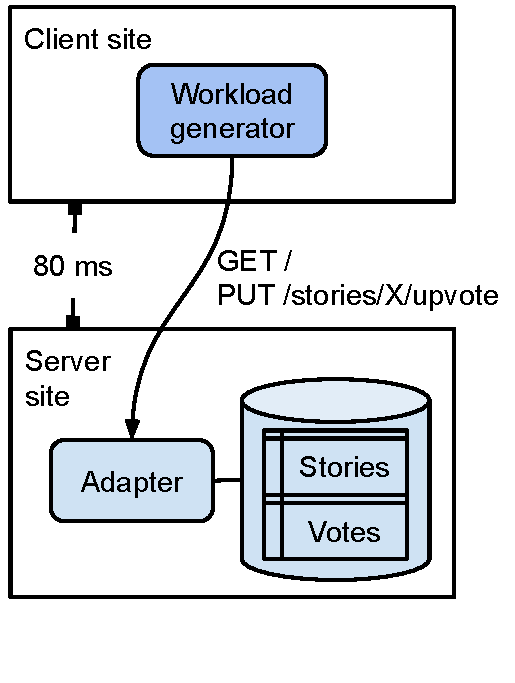
\includegraphics[width=\textwidth]{./figures/evaluation/evaluation_deployments_baseline_remote.pdf}
            \caption{Baseline/remote}
            \label{fig:deployments_baseline_remote}
        \end{subfigure}
        \hfill
        \begin{subfigure}[b]{0.24\textwidth}
            \centering
            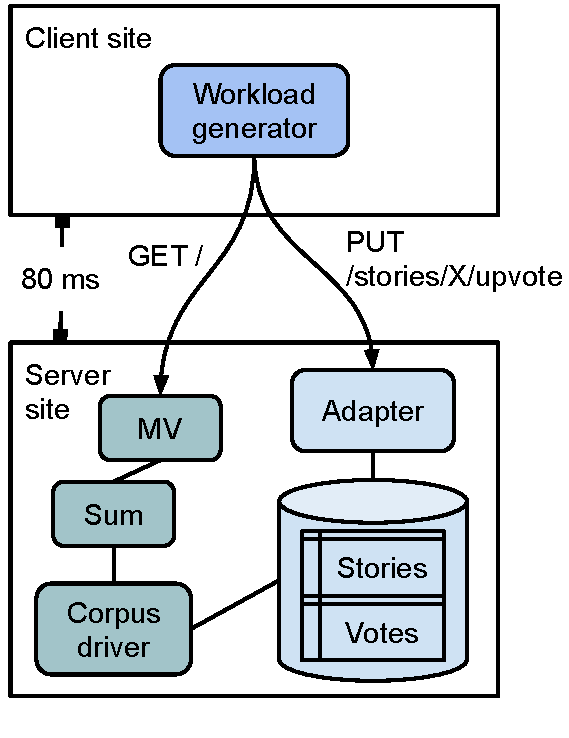
\includegraphics[width=\textwidth]{./figures/evaluation/evaluation_deployments_proteus_remote.pdf}
            \caption{Proteus/remote}
            \label{fig:deployments_proteus_remote}
        \end{subfigure}
        \hfill
        \begin{subfigure}[b]{0.24\textwidth}
            \centering
            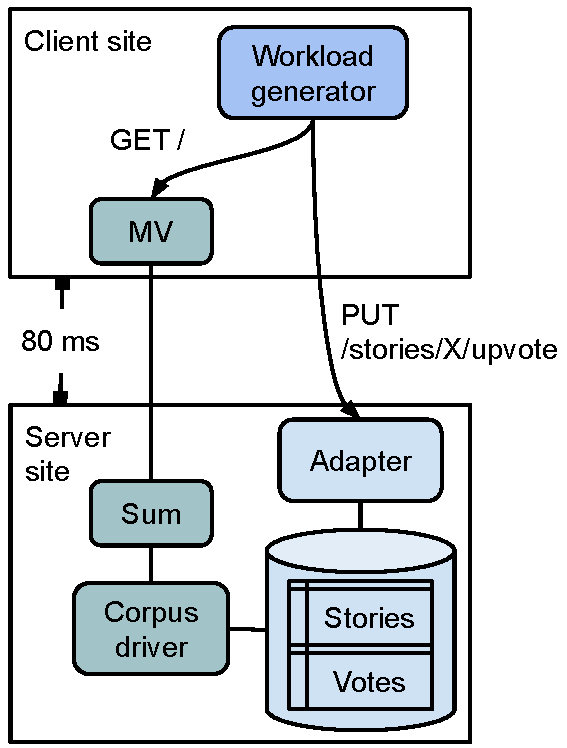
\includegraphics[width=\textwidth]{./figures/evaluation/evaluation_deployments_proteus_local.pdf}
            \caption{Proteus/local}
            \label{fig:deployments_proteus_local}
        \end{subfigure}
        \hfill
        \begin{subfigure}[b]{0.24\textwidth}
            \centering
            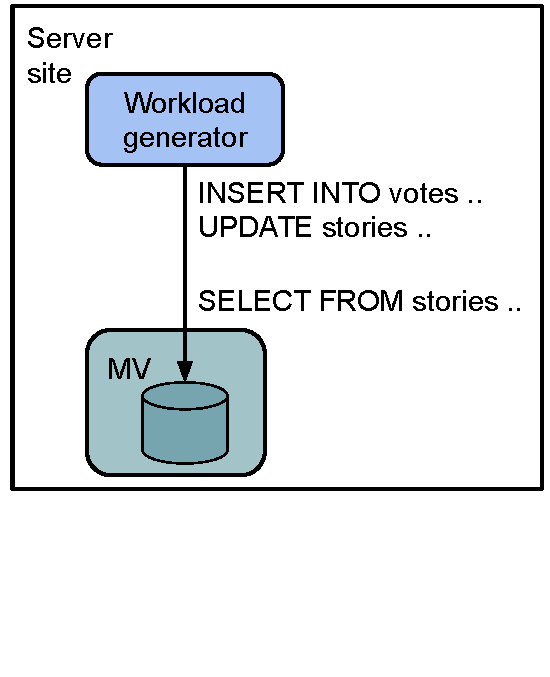
\includegraphics[width=\textwidth]{./figures/evaluation/evaluation_deployments_internal.pdf}
            \caption{Materialized-view-internal}
            \label{fig:deployments_mv_internal}
        \end{subfigure}
        \caption{Deployments used in this evaluation.}
        \label{fig:eval_deployments}
    \end{figure}

We compare three deployments that differ in how they store and calculate the per-story vote count,
and how they distribute computations and state across the nodes of the system (Figure~\ref{fig:eval_deployments})
\textbf{Baseline/remote} (Fig.~\ref{fig:deployments_baseline_remote}) is equivalent to the real Lobsters application:
it pre-computes and stores vote counts in a column of the Lobsters $stories$ table.
This serves as the baseline approach.
\textbf{Proteus/remote} (Fig.~\ref{fig:deployments_proteus_remote}) consists of the QPU graph shown in Figure~\ref{fig:eval_lobsters_qpu_arch},
deployed on the server site.
In \textbf{Proteus/local} (Fig.~\ref{fig:deployments_proteus_local}),the Materialized view QPU is deployed on the client site.
This is intended to evaluate the effect of placing the materialized view close the client.
We also compare with a deployment (\textbf{Materialized-view-internal}, Fig~\ref{fig:deployments_mv_internal}) in which the workload generator
directly issues request to the Materialized view QPU's state, bypassing the QPU's gRPC server
(the workload generator and materialized view are co-located on the same server).
This aims at providing an indication of the best performance the Materialized view QPU can achieve,
without taking into account its gRPC server (which we have identified as a performance bottleneck).

\begin{figure}[H]
\centering
  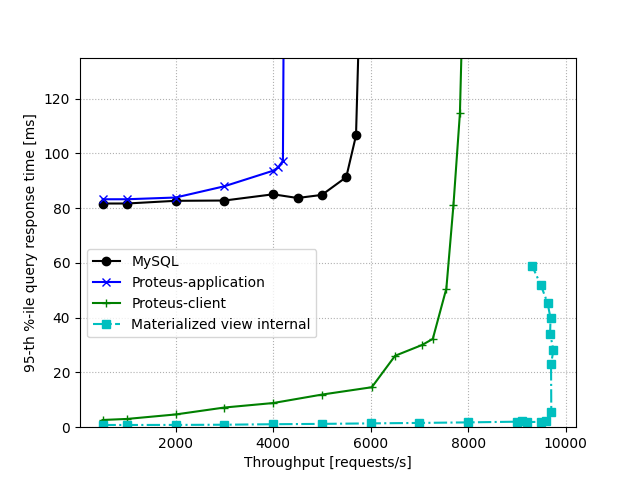
\includegraphics[width=0.7\textwidth]{./figures/evaluation/responseTime.png}
  \caption{Throughput vs 95th percentile query response time.}
  \label{fig:responseTime}
\end{figure}

Figure~\ref{fig:responseTime} shows throughput--query response time plots of these deployments.
The ideal throughput--response time curve would be a horizontal line with low response time.
The lower bound response time for Baseline/remote and Proteus/remote is 80 ms as this is the round-trip time between sites.
In reality, all systems' plots have a ``hockey stick'' shape:
latency remains relatively low until a point in which the system fails to keep up with the offered load.
After that point, the system cannot achieve additional throughput, and response time increases.

Materialized-view-internal scales up to 9800 requests/second,
outperforming both Proteus deployments.
This deployment is intended to evaluate the performance of the core functionality of the Materialized view QPU,
by directly translating front page and vote operations to accesses to the QPU's state using a thread pool,
bypassing the client-server gRPC communication.
Because of that, we conclude that the gRPC communication incurs a significant overhead in the throughout that
can be achieved by the system.

Proteus/remote scales to 4200 requests/second, which is a 24\% overhead compared to the baseline deployment (Baseline/remote),
which scales to 5500 requests/second.
Both those deployments eventually read and write state to a MariaDB instance.
The difference is how they translate requests to database accesses.
The adapter used in the Baseline/remote deployment uses a simple logic that translates vote and front page request to database transactions.
Conversely, the Materialized view QPU used in the Proteus/remote deployment contains more complex logic,
such as parsing received queries in SQL form, and receiving records from its input stream and updating the materialized view.
We attribute the observed 24\% overhead to the more complex logic.

In the Proteus/local deployment, query response time is significantly lower.
This is achieved because moving the Materialized view QPU to the client site removes the need for a costly round-trip to
the server site, and thus removes the 80 ms lower bound.
In addition, Proteus/local achieves a 28\% increase in achieved throughput compared to the Baseline/remote deployment
(we consider the maximum achieved throughput for which response time does not exceed 20ms and 100ms respectively).
We attribute this improvement to the lower concurrency required to generate the same load in Proteus/local
compared to Proteus/remote and Baseline/remote.
In more detail, offering a certain load (volume of requests/second) requires creating a number of concurrent client threads,
each performing a request.
When the round-trip time between sites is 80 ms, each of these threads executes significantly longer compared to
when the round-trip is just a few milliseconds.
As a result, offering a given amount of load in the Proteus/remote setup results in a significantly greater number
of threads, and thus open connections to the QPU's gRPC server, than in the Proteus/local setup.
If the number of connections that can be opened is not bounded by a connection pool, this overloads the QPU's gRPC server,
significantly increasing response times.
When a connection pool is used, each requests needs to wait for an available connection,
again increasing the end-to-end response time experienced by the client.

\medskip
\noindent
\textbf{Conclusion.} Our experiments confirm that placing materialized views closer to the client benefits read-heavy applications
by removing costly round-trip communication across sites, and achieves scalability improvements.
This results is expected, and shows the benefits that can be achieved by enabling this placement.


\subsection{Freshness}
\label{sec:eval_freshness}

\subsubsection{Freshness vs Throughput}
\label{sec:eval_freshness_throughput}

In the actual Lobsters application (and the Baseline/remote deployment),
the vote count is maintained in the $stories$ table.
Because of the consistency guarantees of MariaDB,
the vote count of a story, is always up-to-date with the state of the $votes$ table.
However, maintaining a materialized view placed at a remote site synchronously adds prohibitive overhead to write operations.
Because of that the QPU graph in this evaluation maintains the materialized view asynchronously, and, as a result,
its state might be stale relative to the state of the corpus.

In this section, we present, for the experiments describe in the previous section,
the measurements for the freshness metrics presented in Section~\ref{sec:eval_setup} (update latency and returned version).
Our aim is to examine the effect of asynchronous derived state maintenance in the freshness of query results.
We present results for both placement schemes (Proteus/local and Proteus/remote).
Query results for the Baseline/remote deployment are always up-to-date,
and update latency is 0.


\begin{figure}[H]
\centering
  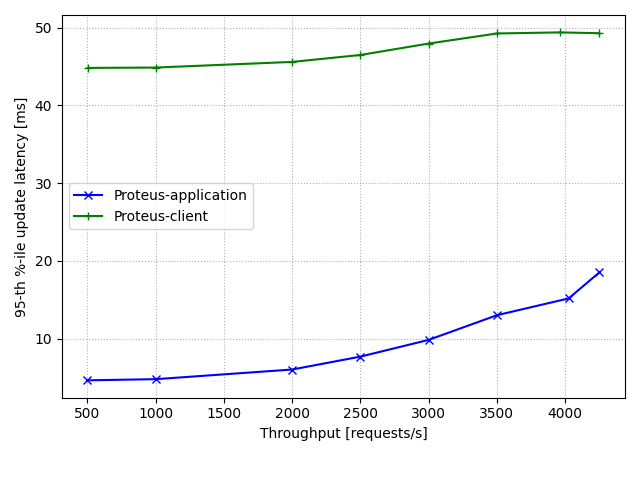
\includegraphics[width=0.7\textwidth]{./figures/evaluation/fr_latency_throughput.png}
  \caption{Throughput vs 95th percentile update latency.}
  \label{fig:fr_latency_throughput}
\end{figure}

Figure~\ref{fig:fr_latency_throughput} shows 95th percentile update latency as throughput increases,
for the Proteus/remote and Proteus/local deployments.
As described above, update latency is the delay between committing a vote in the Lobsters database,
and the corresponding vote count update in the materialized view.
The ideal throughput--update latency curve would be a horizontal line with latency close to the lower bound defined by
the communication latency.
The lower bound for Proteus/remote is 40 ms while for Proteus/local it is less than 1ms.
In reality, latency remains low as long as the system can keep up with the offered vote request load,
and then increases.

Results show the Proteus/local setup scales well; Update latency remains within 5-10 ms of the lower bound.
The Proteus/remote setup exhibits a higher update latency:
For 4250 requests/second, the update latency in Proteus/remote is 88\% higher than in Proteus/local,
relative to the lower bound.
This can be attributed to the same reasons as the scalability difference between the two deployments:
The Materialized view QPU in Proteus/remote is more loaded because more connections are concurrently ongoing
for the same load value, compared to Proteus/local,
leading to increased latency for applying updates to the view.

\begin{figure}[H]
\centering
  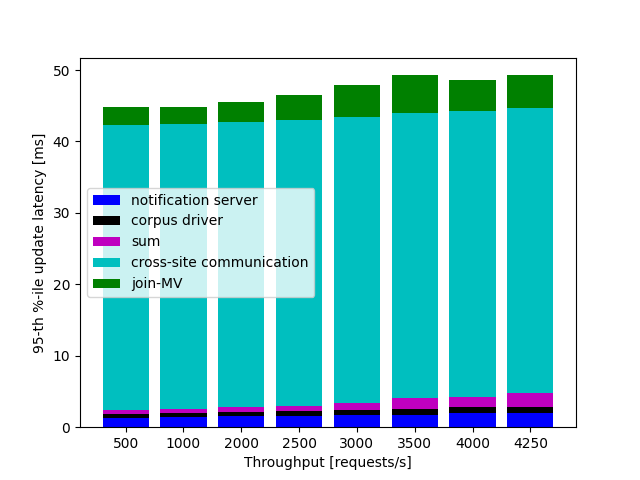
\includegraphics[width=0.7\textwidth]{./figures/evaluation/fr_latency_throughput_breakdown.png}
  \caption{Breakdown of 95th percentile update latency in the Proteus/local deployment
  (as shown in Figure~\ref{fig:fr_latency_throughput}) as throughput increases.}
  \label{fig:fr_latency_throughput_breakdown}
\end{figure}

Each vote committed in the database triggers a record that flows through the QPU graph, and eventually updates the corresponding
vote count in the Materialized view QPU.
Figure~\ref{fig:fr_latency_throughput_breakdown} shows a breakdown of the update latency in the Proteus/local
deployment.
It depicts the delay at each step that vote records follow through the QPU graph.

A vote record's path consists of the following steps:
\begin{enumerate}
  \item When the transaction that inserts a vote record into the Lobsters database commits,
  a trigger sends a message to the notification server (Section~\ref{sec:implementation}).
  The notification server then constructs an update record and sends it to the Corpus Driver QPU through a gRPC stream.
  The duration of this step is shown as \textbf{notification server} in Figure~\ref{fig:fr_latency_throughput_breakdown}.

  \item The Corpus driver receives an update record, and forwards it to the Sum QPU (\textbf{corpus driver}).

  \item The Sum QPU receives an update record, computes an updated vote count,
  and sends a corresponding record to the Join QPU (\textbf{sum}).

  \item \textbf{Cross-site communication} in Figure~\ref{fig:fr_latency_throughput_breakdown} corresponds to the delay for
  sending an update record from the Sum QPU, located at the server site, to the Join QPU, located at the client site.

  \item Finally, the Join QPU receives a record and updates the materialized view accordingly (\textbf{join-MV}).

\end{enumerate}

We observe that:
\begin{itemize}
  \item Update latency is dominated by cross-site communication  (up to 89\%).
  \item Latency at the Corpus driver and Sum QPUs is low: 2ms and 6ms at most.
  This is expected: the Corpus driver simply forwards records upstream;
  The Sum QPU, for each record, updates a vote count stored in memory, and sends a record upstream.
  \item Latency at the notification server and Materialized View QPU increases as the offered load increases.
  However, both scale well as the load increases.
  For the Materialized view QPU this is due to the increasing load in the database that stores the materialized view.
  The latency increase in the notification server can be attributed to the increased load in the database,
  resulting in more triggers being executed concurrently.
\end{itemize}

\begin{figure}[H]
\centering
  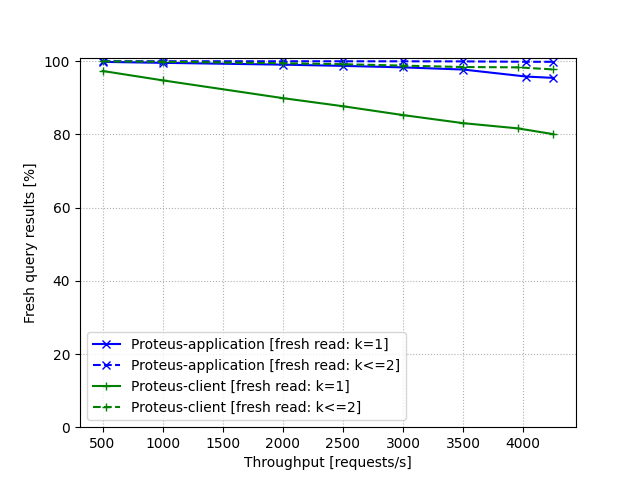
\includegraphics[width=0.7\textwidth]{./figures/evaluation/fresh_reads_throughput.png}
  \caption{Throughput vs percentage of query results and that return a fresh version.
  A returned result is considered fresh if 1) it is the most up-to-date version committed in the database at that time (k=1),
  2) it is amongst the two most up-to-date versions committed in the database at that time (k$\leq$2).}
  \label{fig:fresh_reads_throughput}
\end{figure}

\bigskip
\noindent
Figure~\ref{fig:fresh_reads_throughput} shows the freshness of query results as throughput increases,
measured as the percentage of query results that returned fresh versions.
We define a returned result as a single story with its vote count;
Each front page request returns 25 stories, and each is considered separately.
We consider a scenario in which only the most latest version is considered fresh (k=1),
and one in which the two most recent versions are considered fresh (k$\leq$2).

We observe that:
\begin{itemize}
  \item Proteus/remote has better freshness than Proteus/local, as expected.
  For the k=1 scenario, over 95\% of reads observe the latest versions under the highest load.
  For the k$\leq$2 scenario, freshness remains nearly constant at over 99\%.
  \item Freshness in Proteus/local decreases as throughput increases.
  Proteus/local suffers from up to 80\% stale query results (for k=1), and freshness decreases constantly as load increases.
  However, most stale results observe the second most up-to-date version:
  in the k$\leq$2 scenario over 97\% of query results are fresh.
\end{itemize}

These results can be explained using Figure~\ref{fig:fr_latency_throughput}.
In Proteus/local, it takes at least 45 ms for an updated vote count to be reflected in the materialized view,
but a front page request reaches the view with significantly lower delay.
When load is low, this does not lead to stale query results because there are a few vote requests (5\%).
However, as load increases, queries observe increasingly more stale materialized view  entries.

This is not the case for Proteus/remote.
There, both types of requests reach the materialized view with similar delay,
and because of the query-heavy nature of the workload,
most queries observe tha latest materialized view entries.

\begin{figure}[H]
\centering
  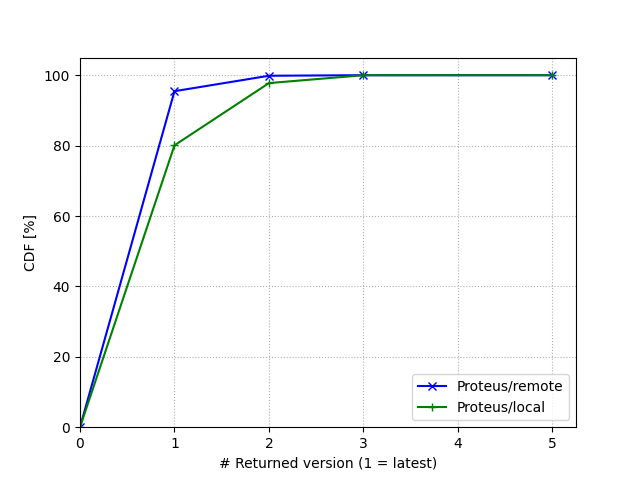
\includegraphics[width=0.7\textwidth]{./figures/evaluation/readV_cdf_throughput.png}
  \caption{CDF of returned version at 4250 requests/second for the Proteus/remote and Proteus/local deployments.}
  \label{fig:readV_cdf_throughput}
\end{figure}

Figure~\ref{fig:readV_cdf_throughput} displays a CDF showing how stale a result of a front page request is
(measured in number of versions),
under a load of 4250 requests/second, for the Proteus/remote and Proteus/local deployments.
Results show that:
\begin{itemize}
  \item In both deployments, most queries return the latest or second most recent version.
  \item Proteus/remote has better freshness than Proteus/local:
  Under the same conditions, Proteus/remote exhibits 4.5\% stale returned results,
  while Proteus/local 20\% (4.4X).
  However, in Proteus/local only 2.2\% of queries results are more stale than the second most recent version.
\end{itemize}

\medskip
\noindent
\textbf{Conclusion.}
Placing the materialized view close to the client, and thus away from the underlying datastore incurs a freshness penalty:
queries return stale results relative to the results that would have been obtained by querying the database.
However, for the workload characteristics in these experiments,
query results are rarely more stale than the second most recent version.
Moreover, update latency and versions freshness scale well as the system's load increases.
We can argue that the level of freshness shown in these experiments to be achievable when placing materialized views close
to the client is sufficient for many query-heavy applications that tolerate eventual consistency.

\subsubsection{Freshness vs round-trip latency}
\label{sec:eval_freshness_rtt}

The experiments in the previous section evaluated the effect of the query processing state placement under a constant
round-trip delay, as the load offered to the system increases.
In this section, we invert these two variables:
we measure freshness under a constant load,
as the (simulated) round-trip time between the application and client site increases,
for the Proteus/local deployment.
The aim of this experiment is to examine the effect of round-trip delay in freshness.

Experiments are performed under a load of 2000 and 4000 requests/second.
We have selected these values based on the results shown in Figure~\ref{fig:fr_latency_throughput}:
Under a load of 2000 requests/second both deployments are able to keep up with the offered load,
while under 4000 requests/second the Proteus/remote scheme exhibits increased update latency.

\begin{figure}[H]
\centering
  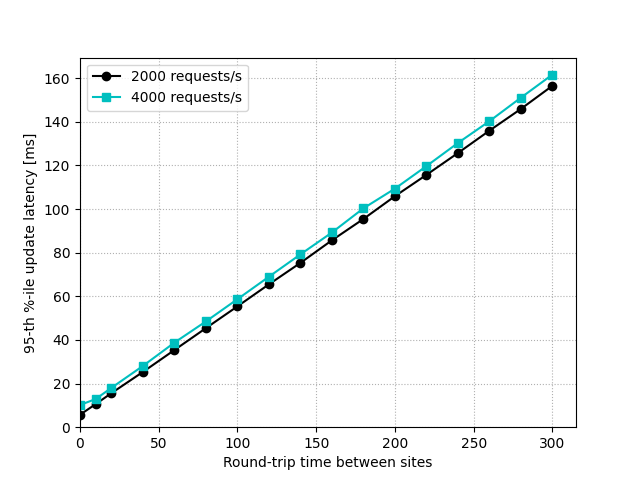
\includegraphics[width=0.7\textwidth]{./figures/evaluation/fr_latency_net_latency.png}
  \caption{Round-trip time between sites vs 95th percentile update latency, for the Proteus/local deployment.}
  \label{fig:fr_latency_net_latency}
\end{figure}

Figure~\ref{fig:fr_latency_net_latency} shows the update latency as the round-trip time between the two sites increases,
under 2000 and 4000 requests/second.
We observe that for both loads, update latency scales linearly with the round-trip time.
Under 2000 requests/second, update latency is at most 5ms above the lower bound set by the one-way network latency
between the two sites, while under 4000 requests/second it is at most 11ms (2.2X).

\begin{figure}[H]
  \begin{subfigure}{0.5\textwidth}
    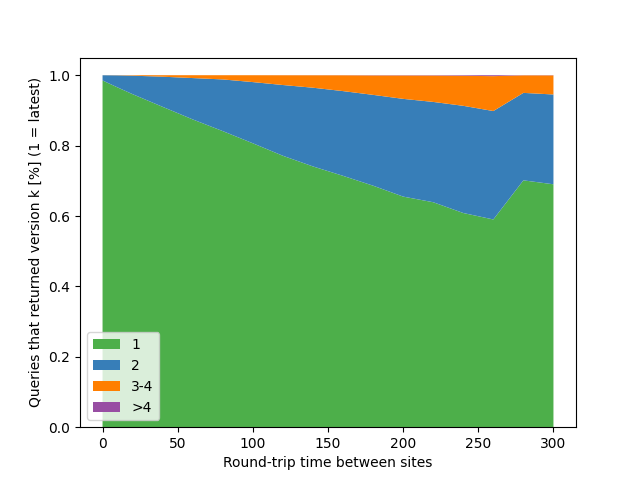
\includegraphics[width=\linewidth]{./figures/evaluation/readV_freshness_netLatency_200.png}
    \caption{2000 requests/second.}
    \label{fig:readV_freshness_netLatency_200}
  \end{subfigure}%
  \hspace*{\fill}
  \begin{subfigure}{0.5\textwidth}
    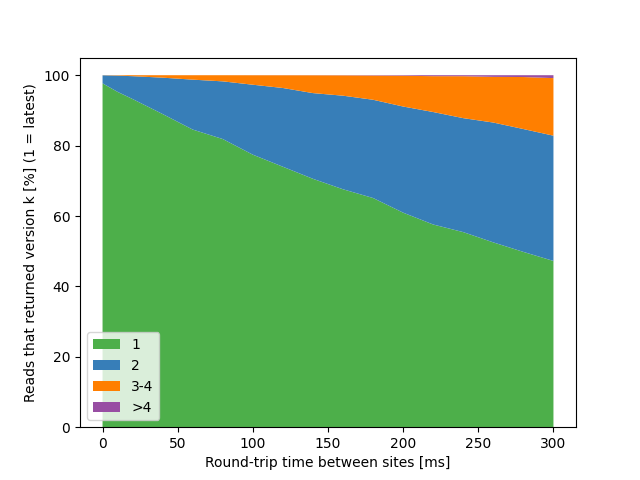
\includegraphics[width=\linewidth]{./figures/evaluation/readV_freshness_netLatency_400.png}
    \caption{4000 requests/second.}
    \label{fig:readV_freshness_netLatency_400}
  \end{subfigure}%
\caption{Distribution of returned version vs round-trip time between sites.}
\label{fig:readV_freshness_netLatency}
\end{figure}

Figures~\ref{fig:readV_freshness_netLatency_200} and~\ref{fig:readV_freshness_netLatency_400}
show the distribution of returned version (which version relative to the most recent one was returned by a query)
for 2000 and 4000 requests/second respectively.
We observe that under both loads freshness decreases as round-trip time increases;
Increasing the load of the system increases the gradient of this decrease.
However, in both cases, queries, generally, observe at most the forth most recent version:
Only 0.06\% and 0.8\% of query results are more stale than the forth most recent version.

\medskip
\noindent
\textbf{Conclusion.}
Update latency, and the freshness of query results are primarily affected by round-trip time between sites,
and to a lesser degree by the system's load.

\subsection{Data transfer between sites}
\label{sec:eval_data_transfer}

\begin{table}[H]
\centering
\begin{tabular}{|c||c|c|c||}
\hline
Deployment & Baseline/remote & Proteus/remote & Proteus/local \\
\hline
Cross-site data transfer (MB) & 0 & 0 & 7.7 \\
\hline
Data transfer out to internet (MB) & $\approx$7700 & $\approx$7700 & $\approx$7700 \\
\hline
\end{tabular}
\caption{Measured data transfer for a 5 minute benchmark with a load of 4000 requests/second.}
\label{tab:data_transfer}
\end{table}

Distributing a query engine across multiple sites entails data transfer between sites.
If the system is deployed on a public cloud platform this incurs an additional cost
because data transfer between data centers is part of public clouds' pricing models.
For example, on AWS EC2, data transfer costs \$0.02 per GB \cite{aws:pricing}.

In the scenario used for these experiments, placing the Materialized view QPU at the client site entails that
update records from the Sum to the Materialized view QPU are sent between sites.

To measure the amount of inter-site data transfer,
we have implemented a mechanism for measuring and aggregating the size of outgoing messages at each QPU.
For a 5 minute benchmark, with 4000 requests/second (200 votes/second), 7.7MB of data were transferred between data centers.
This is because only 5\% of requests are votes, and the size of an update record is small (around 90 bytes),
as it only contains the id and vote count of a story.

In contrast, in the same benchmark, 7.5GB of data were sent as query responses.
This is because the size of a query response is around 4MB
(it contains the records of 25 stories), and 95\% of requests are queries.

We conclude that, in this the evaluation scenario, the materialized view can be placed in the client site without incurring
significant data transfer costs.

\subsection{Conclusion}

The evaluation presented in this section demonstrates that there are benefits and drawbacks to both placement options:
Placing materialized views close to the client results in improvements in response time and throughput,
at the expense of freshness.
Conversely, placing materialized views close to the corpus ensures fresh query results,
but brings limitations to response time and throughput.
As a result, client-site placement of materialized views is more suitable for applications that require low query response times or high
query load, and can tolerate stale query results;
server-site placement is better-suited for applications for which query processing performance is not critical,
but require up-to-date query results.
In addition, evaluation results show that Proteus can to efficiently implement both placement schemes.


\section{Federated metadata search for multi-cloud object storage}
\label{sec:eval_2}

\subsection{Experimental scenario}

The evaluation presented in this section is based on the case study presented in Section~\ref{sec:zenko}.
We consider a multi-cloud data serving system, composed of three storage locations.
A storage location may be a public cloud storage platform (e.g. Amazon S3, Microsoft Azure Blob storage, Google Cloud Storage),
or an on-premise storage system.
Each storage location is independent (not aware of the other locations),
and a multi-cloud data controller (\S\ref{sec:zenko}) is responsible for providing a common namespace across storage locations.
The controller implements an object storage API, such the AWS S3 API:
objects are composed of a primary key, a set of metadata attributes, and content.
This evaluation focuses on providing support for federated queries on metadata attributes.

We consider a system model composed of the 3 storage locations, in 3 geographically distant data
centers.
Each storage location stores a disjoin subset of the dataset.
An instance of the multi-cloud controller is deployed on each storage location,
and users are served by the controller that is geographically closer to their location.
An overview of the system model is shown in Figure~\ref{fig:eval_part2_overview}.

We consider an application that consists of two types of operations:
updating the metadata attributes of a given object,
and performing queries on metadata attributes.

\begin{figure}[H]
\centering
  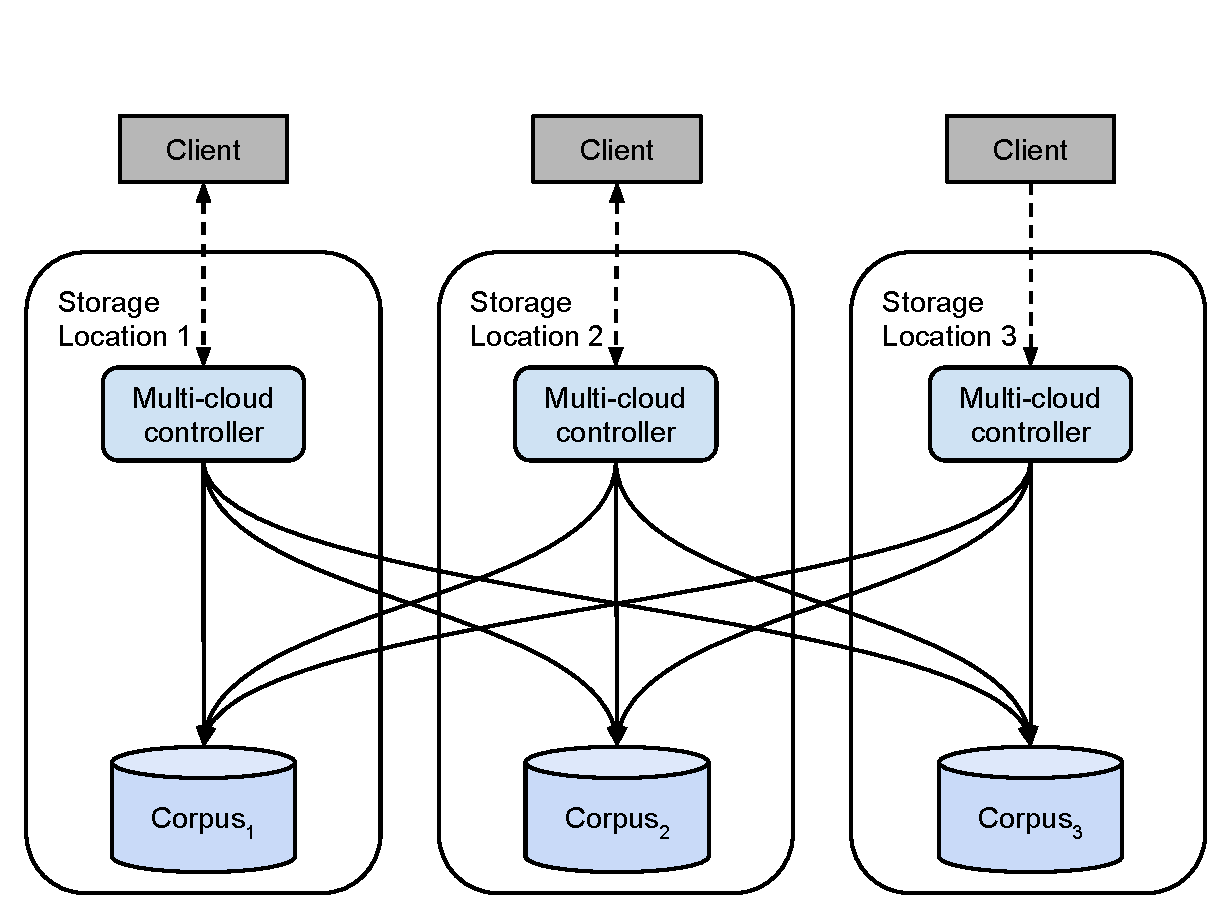
\includegraphics[width=0.7\textwidth]{./figures/evaluation/eval_part2_overview.pdf}
  \caption{An overview of the system model in \S\ref{sec:eval_2}.}
  \label{fig:eval_part2_overview}
\end{figure}

\subsection{Methodology}

As discussed in Section~\ref{sec:zenko}, there are alternative approaches for designing a multi-cloud query engine.
The aim of this evaluation is to demonstrate the need for flexibility in the query engine's design for addressing the
needs of different applications,
and validate that QPU-based query engines can provide the required flexibility.

To achieve that, we consider 3 query engine configurations (QPU graphs), 3 workload types with different query-update ratios,
and 3 metrics (query processing performance, freshness, and data transfer between storage locations);
We experimentally determine which query engine configuration is better-suited for each combination of workload type and target metric.

\bigskip
\noindent
\textbf{Query engine configurations.}
The main functionality of the query engine in this scenario is to maintain secondary indexes for accelerating queries on
metadata attributes.
We consider the following approaches for partitioning and placing a multi-cloud secondary index across the system.

\begin{itemize}
  \item \textbf{Replicated global indexes (rg-index):}
  An index responsible for indexing data from all storage locations is deployed on each location.
  This approach has the advantage that queries are served by the local index.
  However, each index needs to receive update notifications from the two remote storage locations.
  Depicted in Figure~\ref{fig:rg_index}.

  \item \textbf{Partitioned index (p-index):}
  In this configuration, the index on each storage location is responsible for the local corpus.
  The system forwards each query to all 3 storage locations, and combines the retrieved results.
  This approach requires a third of the storage space for indexes compared to rg-index,
  and ensures that update notifications are sent only to the local index,
  at the expense of requiring cross-site communication for serving queries.
  Depicted in Figure~\ref{fig:p_index}.

  \item \textbf{Partitioned index with caching (p-index-cache):}
  This configuration is an extension to p-index that uses a caching layer with the aim of reducing access to remote indexes.
  For each index, a cache responsible for caching sub-query results from it is deployed on the two remote storage locations.
  Depicted in Figure~\ref{fig:p_index_cache}.
\end{itemize}

\begin{figure}[H]
  \begin{subfigure}{0.5\textwidth}
    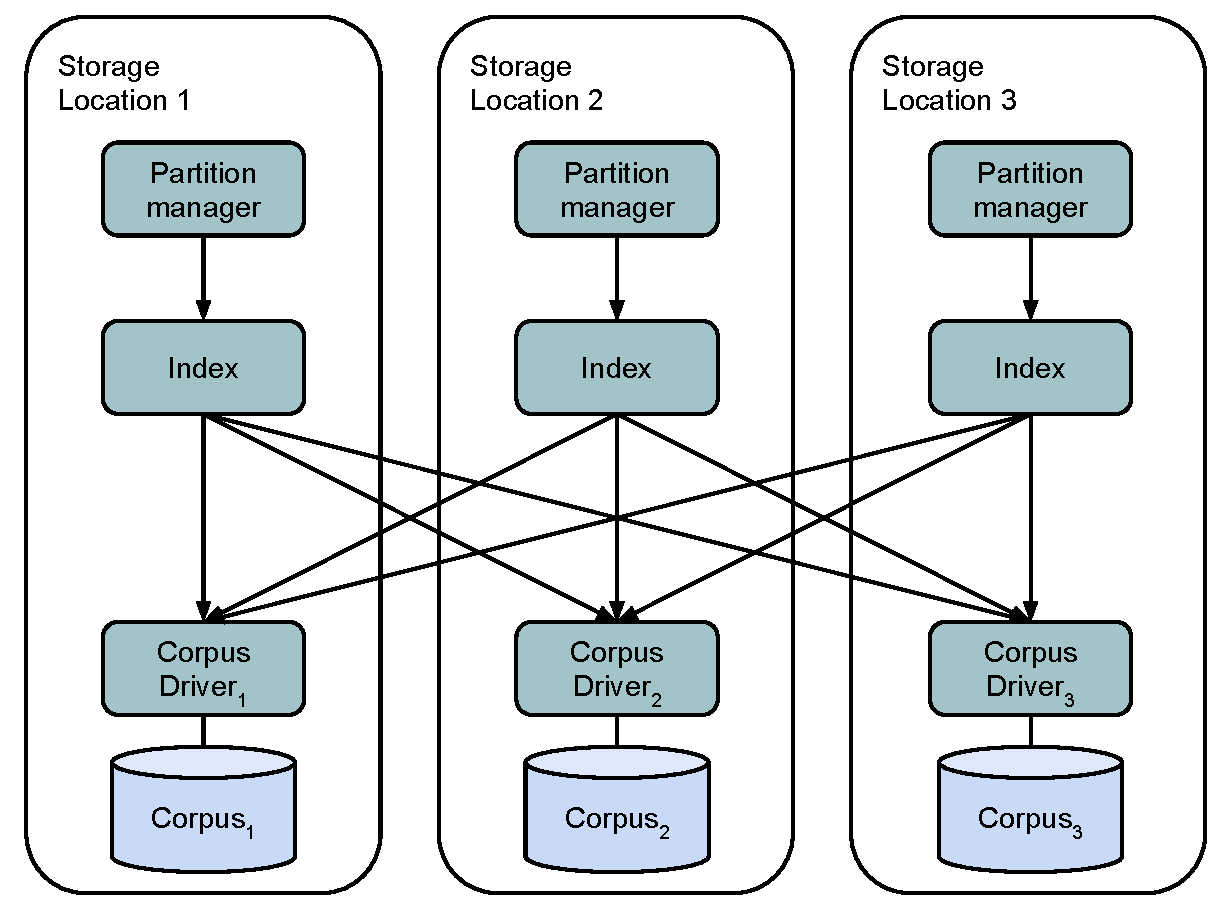
\includegraphics[width=\linewidth]{./figures/evaluation/rg_index.pdf}
    \caption{}
    \label{fig:rg_index}
  \end{subfigure}%
  \hspace*{\fill}
  \begin{subfigure}{0.5\textwidth}
    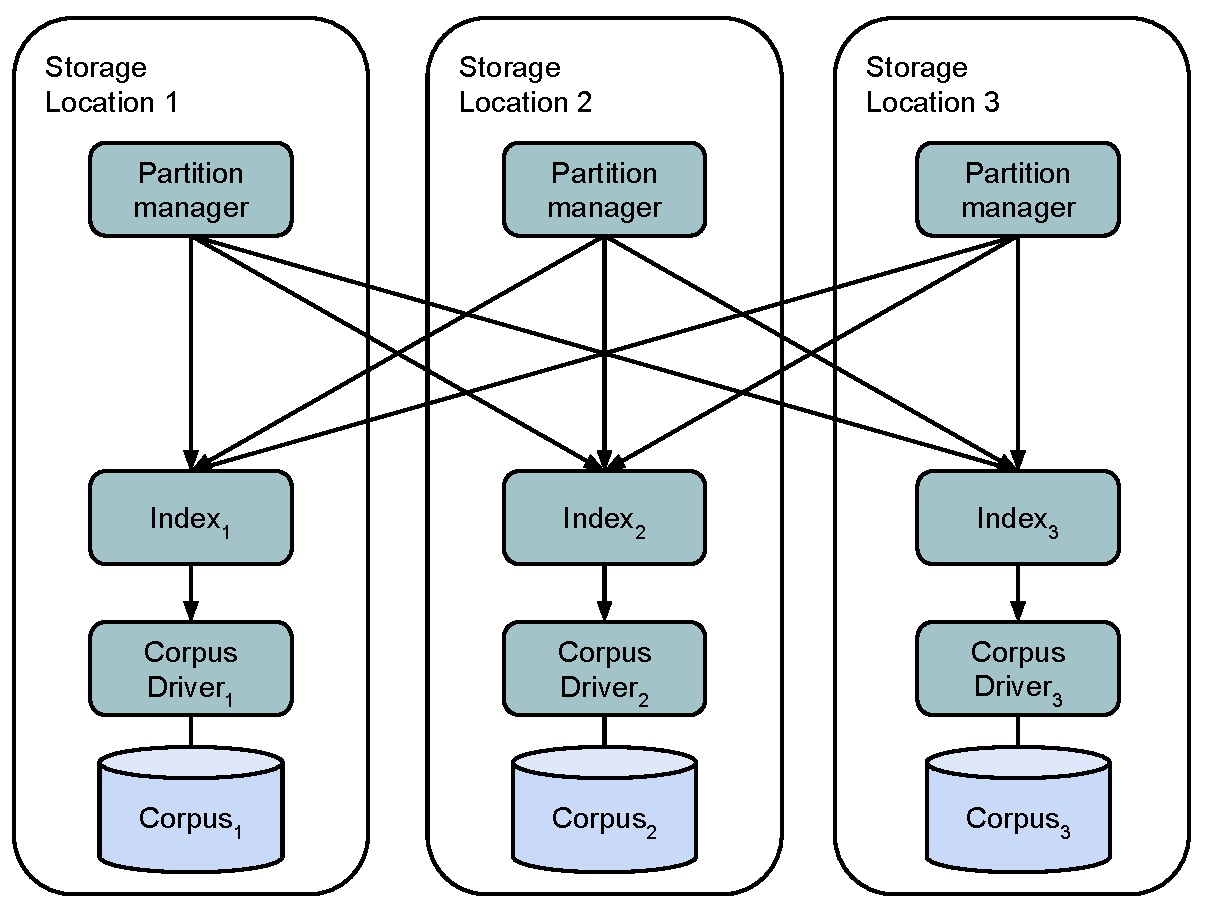
\includegraphics[width=\linewidth]{./figures/evaluation/p_index.pdf}
    \caption{}
    \label{fig:p_index}
  \end{subfigure}%
  \caption{The (a) replicated global indexes (rg-index) and (b) partitioned index (p-index) QPU graph configurations.}
  \label{fig:p_rg_index}
\end{figure}

\begin{figure}[H]
\centering
  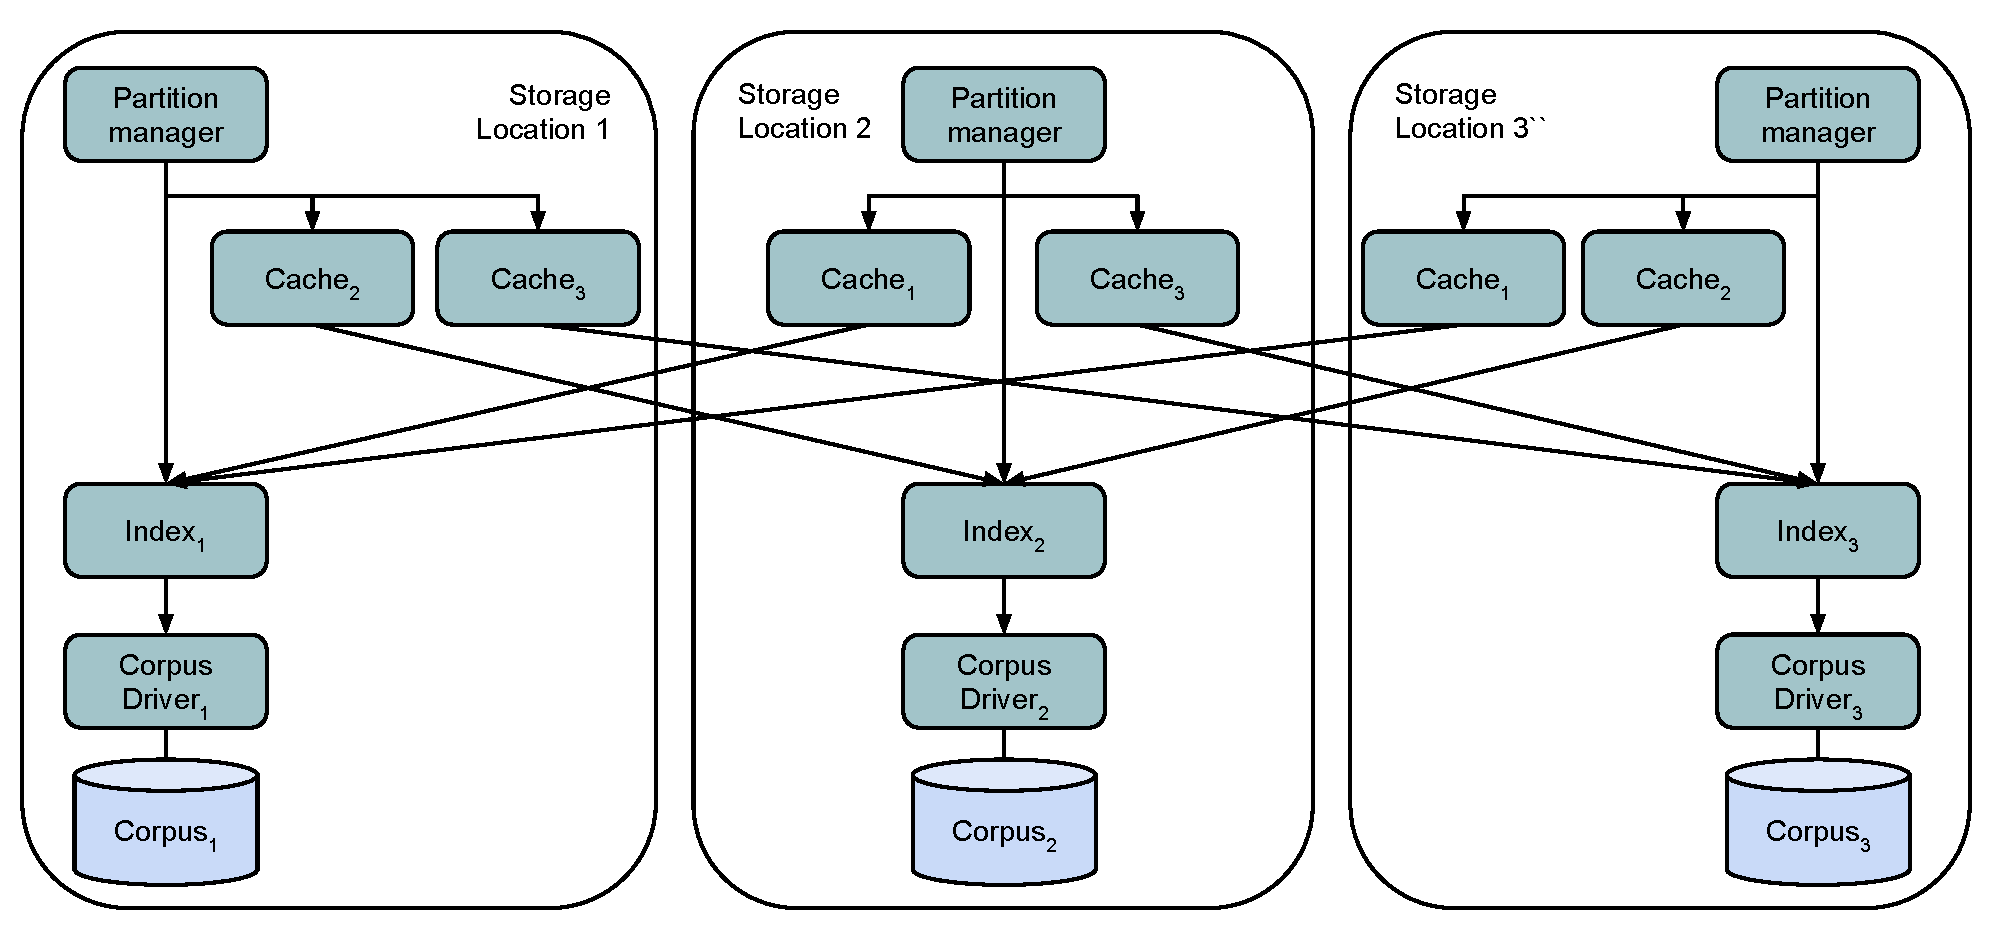
\includegraphics[width=0.7\textwidth]{./figures/evaluation/p_index_cache.pdf}
  \caption{The partitioned index with caching (p-index-cache) QPU graph configuration.}
  \label{fig:p_index_cache}
\end{figure}

\bigskip
\noindent
\textbf{Workload types.}
Overall, we consider a query-heavy application that requires the use of secondary indexes for query processing.
We examine 3 workload types, each with a different mix of query and update operations:
95\% queries - 5\% updates (w95/5), 80\% queries - 20\% update (w80/20),
60\% queries - 40\% update (w60/40).

\bigskip
\noindent
\textbf{Evaluation metrics.}
For this evaluation, we use the metrics discussed in Section~\ref{sec:eval_1}:
query processing performance, freshness and data transfer cost for data transferred between storage locations.

\subsection{Experimental Setup}
On each storage location, data is stored on an instance of MongoDB.
We use MongoDB as an object store:
an object is represented by a MongoDB document, with document fields representing the object's metadata attributes.
At the start of each experiment, we preload each storage location with with 33k objects,
so that in total the system stores 100k objects.

The Index QPU implements an in-memory B-tree secondary index.
The Cache QPU implements a cache with a least recently used (LRU) eviction policy,
and a time-to-live (TTL) based invalidation policy.
We set the size of caches so that each cache can hold 50\% of the index entries it is responsible for,
and configure the TLL value to 5 seconds.

We configure the system so that there is an 80sm round trip time between storage locations in order to
simulate a multi-cloud system deployed over distant geographic locations.

\bigskip
\noindent
\textbf{Workload generation and measurements configuration.}
We use the Yahoo! Cloud Serving Benchmark (YCSB) \cite{ycsb} for generating workload and performing measurements.
The core operation of the YCSB framework is that it drives a number of client threads,
each executing a sequential series of operations by making calls to the underlying system,
and measures the latency and achieved throughput of their operations.
At the end of an experiment, a statistics model aggregates the measurements and reports the achieved throughput and
the measured latency percentiles.

We have modified YCSB's MongoDB driver to send query operations to Proteus.
We deploy a YCSB instance on each storage location.
On each location, YCSB client threads send update operations to the local MongoDB instance,
and query operations to the local Partition Manager QPU.
At the end of an experiment, we gather and aggregate measurements from all three storage locations,
and compute the total achieved throughput and latency percentiles.

Each object in the dataset has multiple, randomly generated metadata attributes.
We ensure that a numeric attribute with a specified key existing in every object.
Query operation in the workload are point queries that refer to this attribute.
Both the attribute's values and query predicated follow a uniform distribution.
We use the mechanism presented in Section \ref{sec:eval_setup} for measuring freshness.

Experiments run for 5 minutes unless otherwise specified, and we start taking measurements after an initial
warmup period of 30 seconds.

\subsection{Query processing performance}

\begin{figure}[H]
\centering
  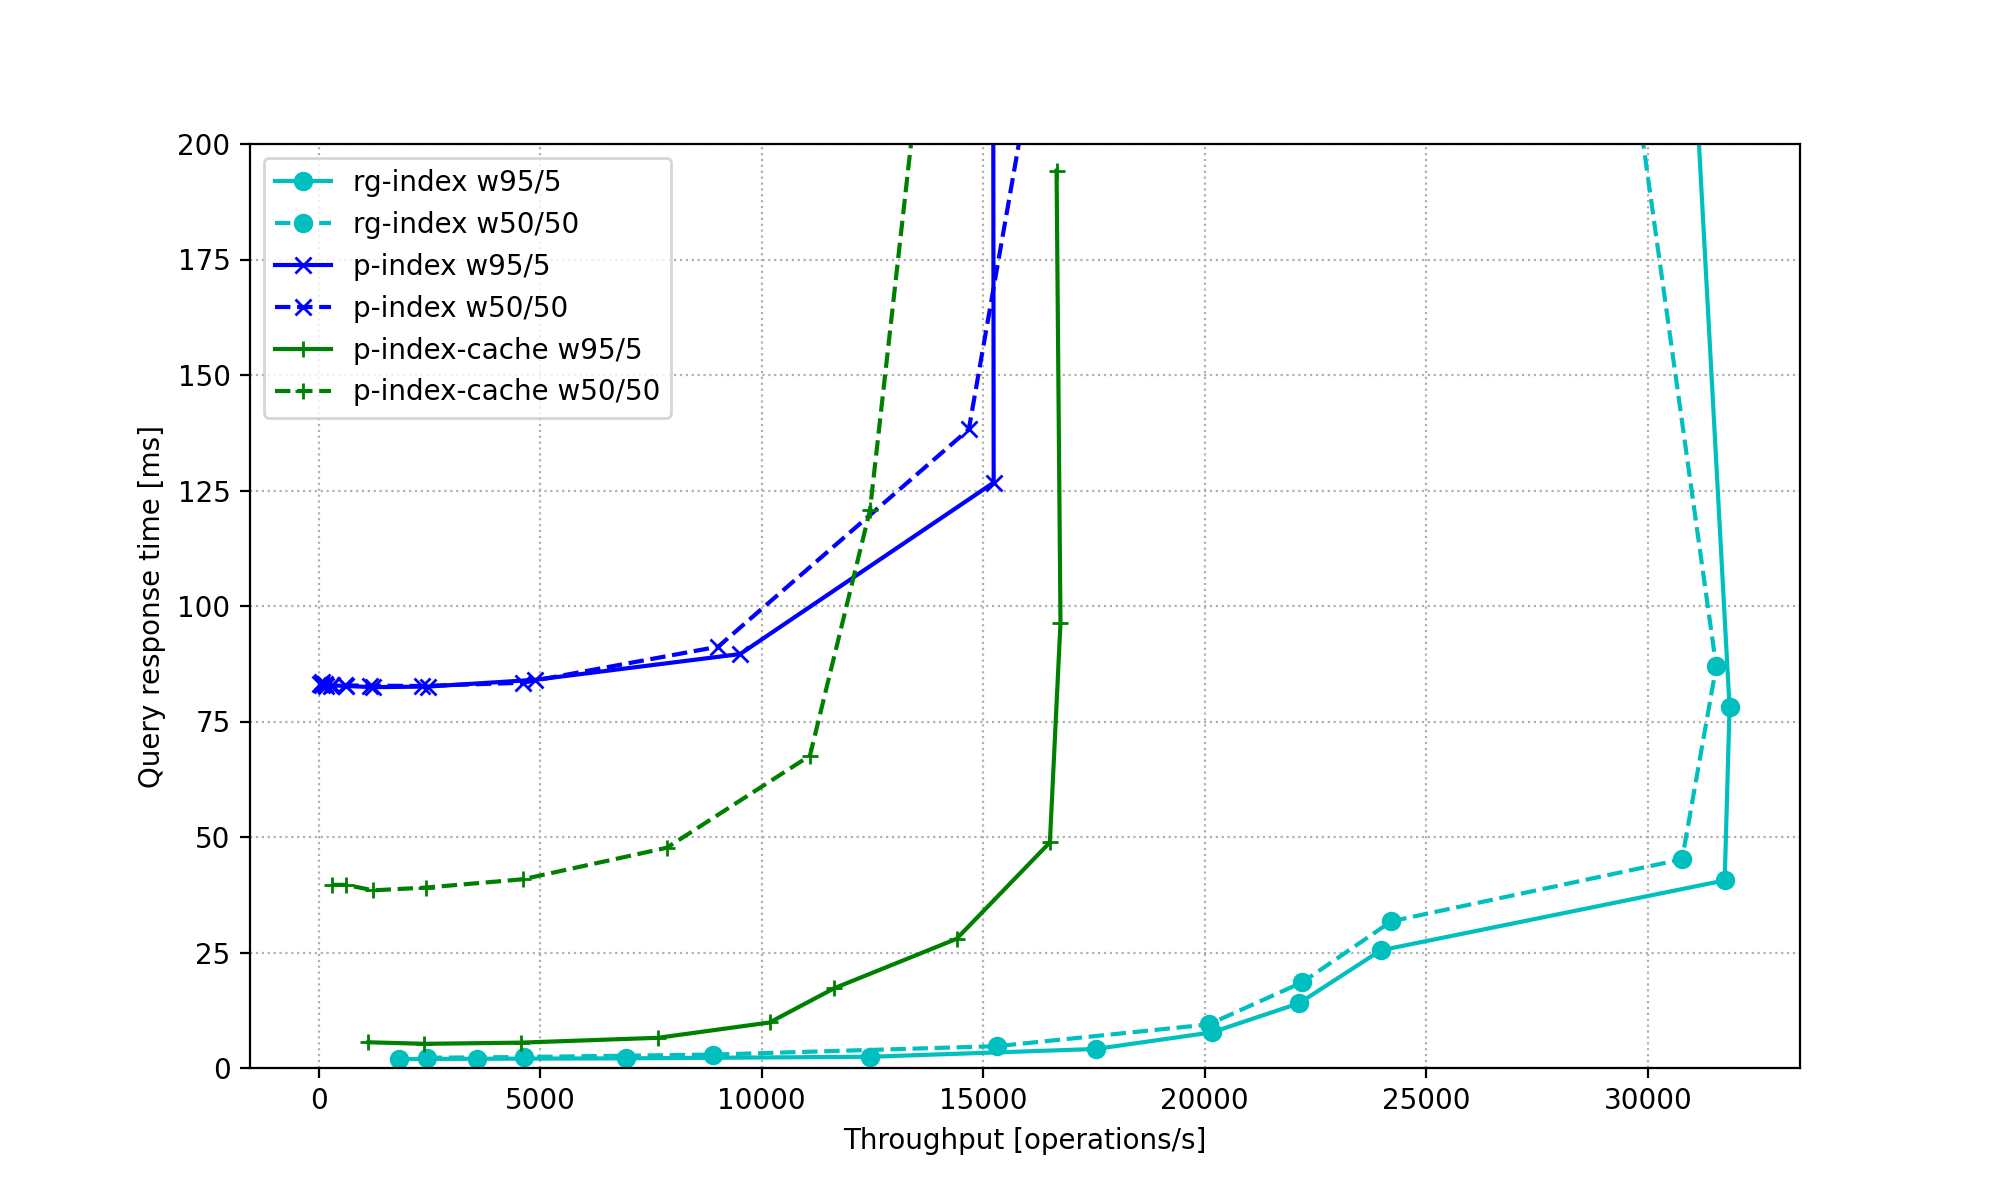
\includegraphics[width=0.9\textwidth]{./figures/evaluation/ycsb_responseTime.png}
  \caption{Throughput vs query response time. Plots for the rg-index and p-index configuration show the 90th percentile response time;
  Plots for the p-index-cache configuration show average response time in order to capture the effect of caching in reponse time.}
  \label{fig:ycsb_responseTime}
\end{figure}

Figure~\ref{fig:ycsb_responseTime} shows throughput--query response time plots for the 3 QPU graph configuration and 3 workload
types.
We observe that:
\begin{itemize}
  \item Response time in the p-index configuration is 80ms higher than in the rg-index configuration.
  This is because in p-index the query engine forwards queries to indexes across storage locations while
  in rg-index queries are served by the local index.
  \item Average response time in the p-index-cache configuration is around 80ms when load is low,
  and then decreases as load increases.
  This effect is the result of caching:
  In low load values, caches are not filled, and most queries result in cache misses;
  As load increases, more queries are served from the cache, decreasing the average query response time.
  \item The p-index configuration achieves around 50\% throughput compared to rg-index.
  This can be attributed to the closed loop workload generation mechanism of YCSB:
  Given a certain number of client threads, in rg-index each query operation has a takes less than 25ms
  when the system is not saturated, while in p-index each query operation take 85-90ms because of the 80ms
  round trip time between storage locations.
  Therefore, in p-index each client thread cannot offer the same load as in rg-index.
  \item The p-index-cache configuration achieves 21\% lower throughput (for the w95/5 workload).
  This is expected as each cache miss adds an 80ms overhead to response time,
  resulting in client threads being able to generate less load.
\end{itemize}

We conclude that the rg-index configuration is better-suited for achieving the best query processing performance.
However, this comes at the expense of memory overhead for maintaining a global index at each storage location.
The rg-index-cache configuration requires achieve query processing performance comparable to rg-index,
and requires 66\% the memory of rg-index (because each cache is configured to 50\% the size of an index).

\subsection{Freshness}

In this section, we examine the query result freshness achieved by the alternative QPU graph configurations.
In order to evaluate the freshness of the different configurations,
we break them down into \textit{placement patterns}, we evaluate the freshness of each placement pattern,
and reason about how placement pattern freshness contributes to the overall freshness of QPU graph configurations.
The placement patterns present in the three QPU graph configurations are shown in Figure~\ref{fig:placement_patterns}.

\begin{figure}[H]
  \begin{subfigure}{0.24\textwidth}
    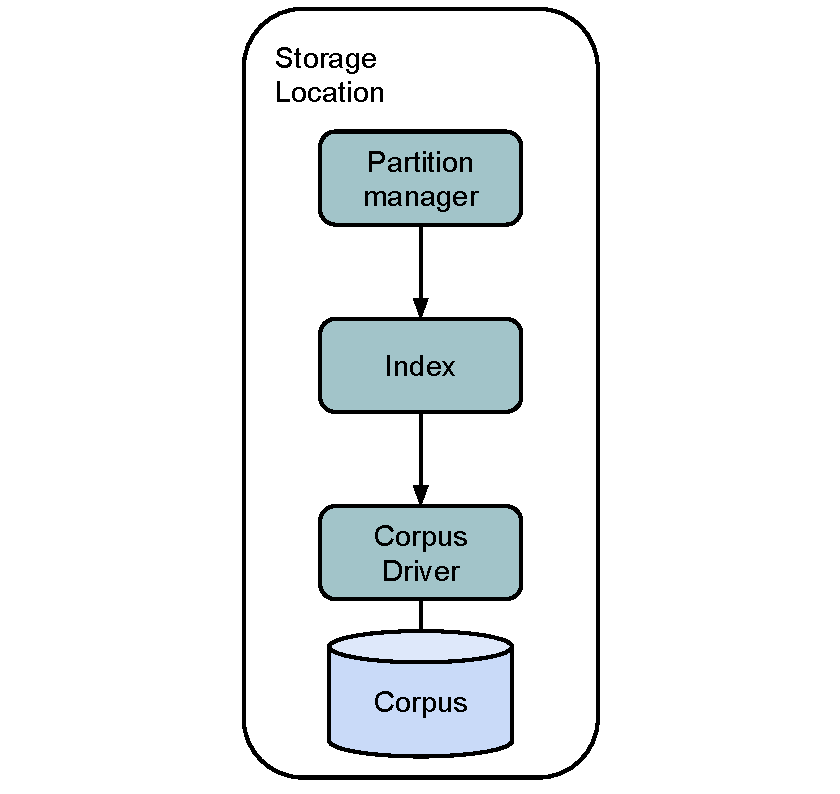
\includegraphics[width=\linewidth]{./figures/evaluation/ycsb_freshness_local.pdf}
    \caption{}
    \label{fig:ycsb_freshness_local}
  \end{subfigure}%
  \hspace*{\fill}
  \begin{subfigure}{0.24\textwidth}
    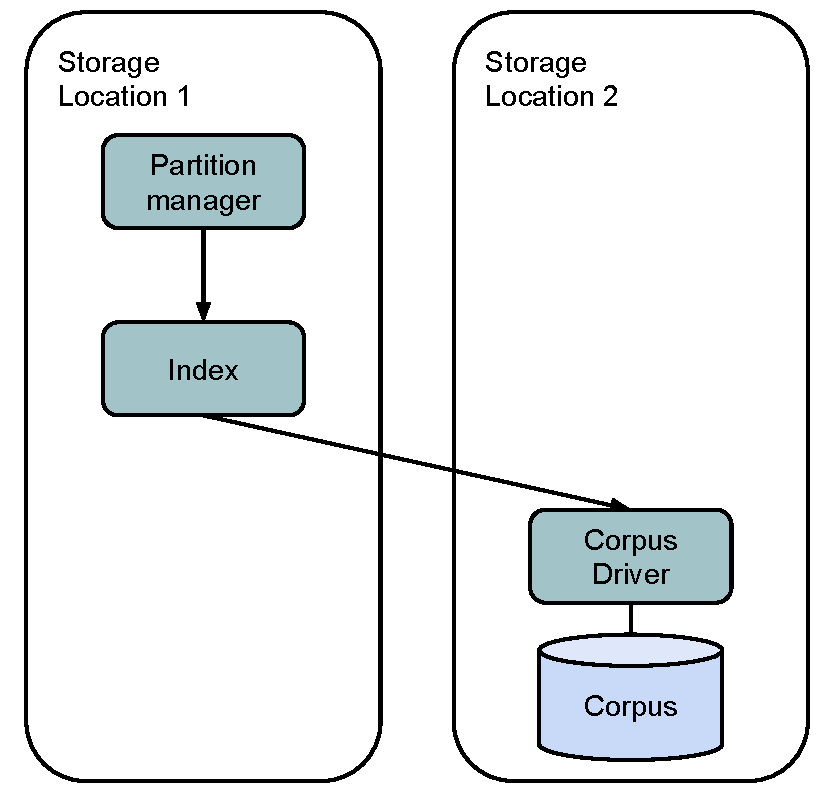
\includegraphics[width=\linewidth]{./figures/evaluation/ycsb_freshness_remote_corpus.pdf}
    \caption{}
    \label{fig:ycsb_freshness_remote_corpus}
  \end{subfigure}%
  \hspace*{\fill}
  \begin{subfigure}{0.24\textwidth}
    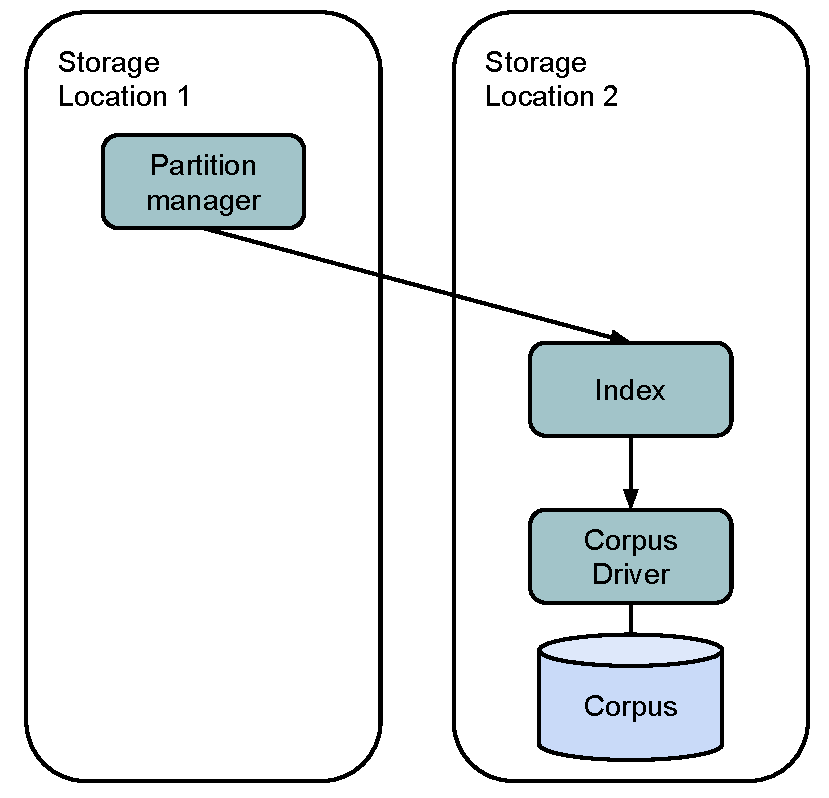
\includegraphics[width=\linewidth]{./figures/evaluation/ycsb_freshness_remote_client.pdf}
    \caption{}
    \label{fig:ycsb_freshness_remote_client}
  \end{subfigure}%
  \hspace*{\fill}
  \begin{subfigure}{0.24\textwidth}
    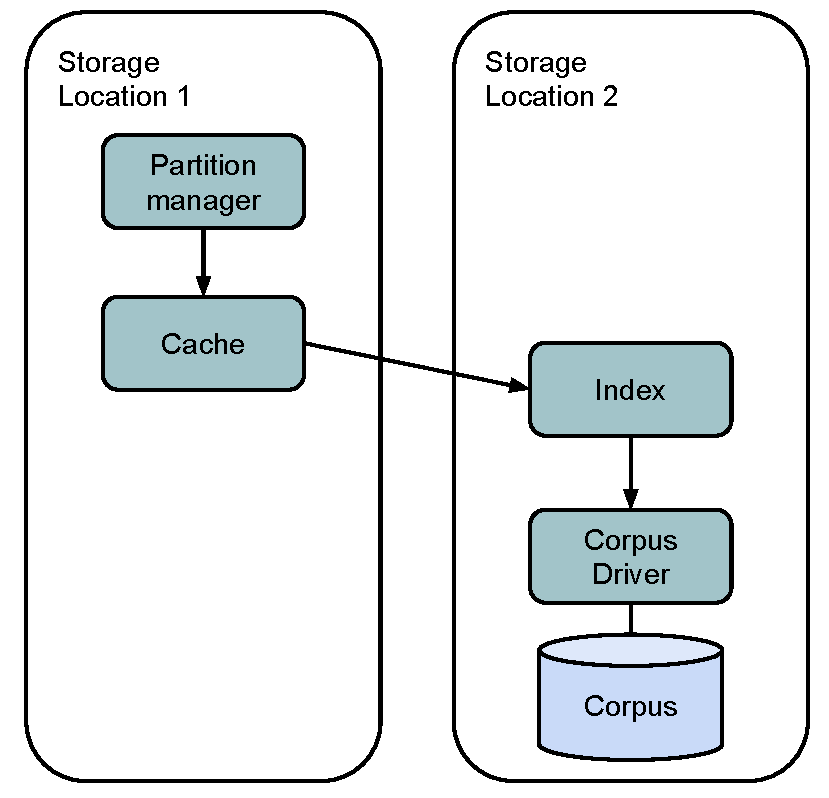
\includegraphics[width=\linewidth]{./figures/evaluation/ycsb_freshness_remote_client_cache.pdf}
    \caption{}
    \label{fig:ycsb_freshness_remote_client_cache}
  \end{subfigure}%
  \caption{Placement patterns. (a) Corpus, index and clients are located on the same storage location (local).
  (b) The corpus is located on a remote storage location (remote-corpus). (c) The index is co-located with the corpus;
  clients are located on a remote storage location (remote-client). (d) A cache is used to reduce cross-location communication (remote-client-cache).}
  \label{fig:placement_patterns}
\end{figure}

\begin{table}[H]
\centering
\begin{tabular}{|c||c|c|c|c||}
\hline
& local & remote-corpus & remote-client & remote-client-cache \\
\hline
rg-index & $\blacksquare$ & $\blacksquare$ &  & \\
\hline
p-index & $\square$ & & $\blacksquare$ & \\
\hline
p-index-cache & $\square$ & &  & $\blacksquare$ \\
\hline
\end{tabular}
\caption{Placement patterns that QPU graph configurations are composed of.
$\blacksquare$ $\blacksquare$ indicates that both patterns contribute to the configuration's freshness.
$\square$ $\blacksquare$ indicated that only the pattern with $\blacksquare$ contributed to the configuration's freshness.}
\label{tab:placement_patterns}
\end{table}

Table \ref{tab:placement_patterns} shows the placement patterns used for each QPU graph configuration.
In rg-index, each index is connected to both local (\ref{fig:ycsb_freshness_local}) and remote (\ref{fig:ycsb_freshness_remote_corpus}) corpus.
As a result, query result freshness is affected by the freshness characteristics of both patterns.
In p-index, each Partition Manager QPU is connected to the the local index (\ref{fig:ycsb_freshness_local}),
and two remote indexes (\ref{fig:ycsb_freshness_remote_client}).
The Partition Manager forwards a given query to all three indexes and waits to receive all responses before responding to
the client.
Because of that, the freshness of p-index is determined by the freshness of the remote-client pattern.
Similarly, the freshness of p-index-cache is determined by the freshness of the remote-client-cache pattern
(\ref{fig:ycsb_freshness_remote_client_cache}).


\begin{figure}[H]
  \begin{subfigure}{0.5\textwidth}
    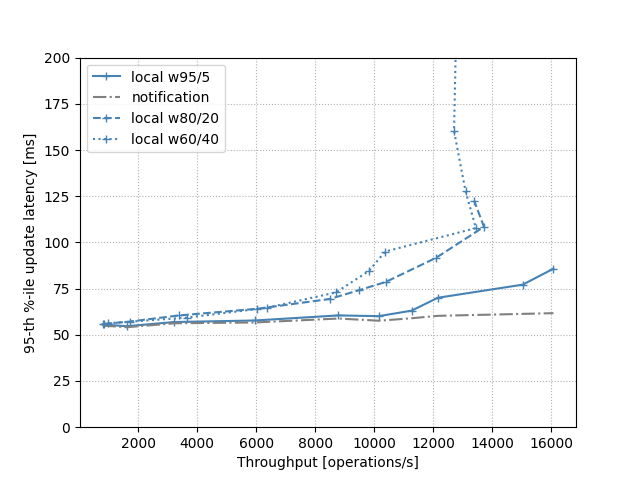
\includegraphics[width=\linewidth]{./figures/evaluation/ycsb_update_latency_local.png}
    \caption{}
    \label{fig:ycsb_update_latency_local}
  \end{subfigure}%
  \hspace*{\fill}
  \begin{subfigure}{0.5\textwidth}
    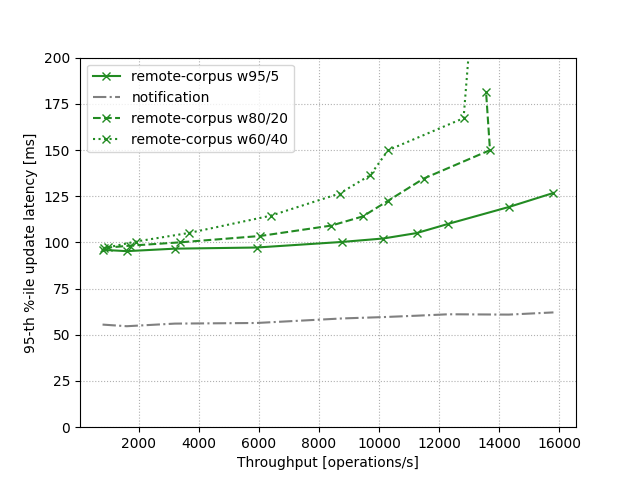
\includegraphics[width=\linewidth]{./figures/evaluation/ycsb_update_latency_remote.png}
    \caption{}
    \label{fig:ycsb_update_latency_remote}
  \end{subfigure}%
  \caption{Throughput vs 95th percentile update latency for the Index QPU in the local (a) and remote-corpus (b) placement patterns.}
  \label{fig:ycsb_update_latency_local_local_remote}
\end{figure}

Figures~\ref{fig:ycsb_update_latency_local} and~\ref{fig:ycsb_update_latency_remote} show the 95th percentile update latency as throughput increases,
for local (\ref{fig:ycsb_update_latency_local}) and remote-corpus (\ref{fig:ycsb_update_latency_remote}) placement patterns.

We implement the storage tier's Subscribe API (\S\ref{sec:storage_tier_api}) using MongDB's change stream functionality \cite{mongo:changestreams}.
Our results show that, with the configuration used for these experiments, the change stream client receives a notification with a 50-60ms delay.
We indicate this as the baseline update latency in the plots (notification).

In addition, we note that our mechanism for measuring update latency includes in update latency
the response time of the update operation performed by the client.
Because update operation response time increases with load, part of the increase in update latency is due to the update operation response time.
Update operation response time is shown in Figure~\ref{fig:ycsb_write_latency}.

\begin{figure}[H]
\centering
  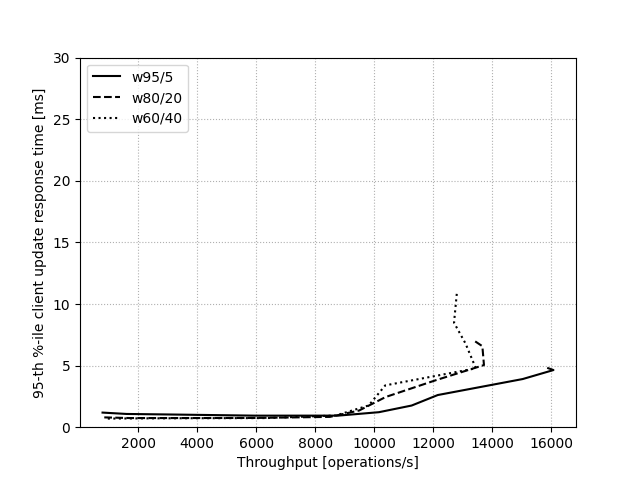
\includegraphics[width=0.7\textwidth]{./figures/evaluation/ycsb_write_latency.png}
  \caption{Throughput vs client update response time. Client updates are always local,
  as in all configurations clients write to the local MongoDB instance.}
  \label{fig:ycsb_write_latency}
\end{figure}

\noindent
For the update latency results in Fig.~\ref{fig:ycsb_update_latency_local_local_remote}, we observe that:
\begin{itemize}
  \item In remote-corpus, update latency is at least 40ms higher that the baseline
  due to the 40ms network latency between storage locations.

  \item Update latency increases with the ratio of updates.
  This is due to contention, as each update needs to acquire a write lock on the index.
  For both placement patterns, for the w80/20 and w60/40 workloads,
  update latency does not scale to loads larger than 13k operations/second.
\end{itemize}

The evaluation results shown in Figures~\ref{fig:ycsb_responseTime} and~\ref{fig:ycsb_update_latency_local_local_remote} demonstrate the trade-off betwee
query performance and query result freshness.
The rg-index configuration, in which queries are served locally, achieves better query processing performance at the expense of increased update latency;
The update latency overhead is determined by the network communication latency between storage locations.
Conversely, the p-index configuration ensures low update latency at the expense query processing performance.
\begin{figure}[H]
  \begin{subfigure}{0.5\textwidth}
    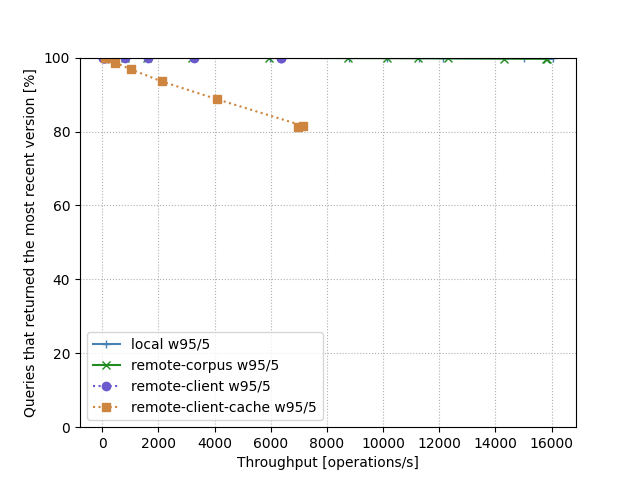
\includegraphics[width=\linewidth]{./figures/evaluation/ycsb_readV_freshness_throughput_9505.png}
    \caption{}
    \label{fig:ycsb_readV_freshness_throughput_9505}
  \end{subfigure}%
  \hspace*{\fill}
  \begin{subfigure}{0.5\textwidth}
    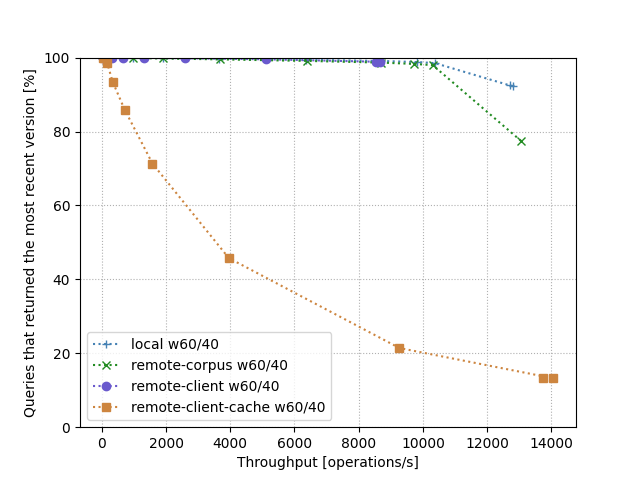
\includegraphics[width=\linewidth]{./figures/evaluation/ycsb_readV_freshness_throughput_6040.png}
    \caption{}
    \label{fig:ycsb_readV_freshness_throughput_6040}
  \end{subfigure}%
  \caption{Throughput vs percentage of queries that returned the most recent version in the w95/5 (a) and w60/40 (b) workload.}
  \label{fig:ycsb_readV_freshness_throughput}
\end{figure}

Next, we examine how update latency affects query result freshness.
Figures~\ref{fig:ycsb_readV_freshness_throughput_9505} and~\ref{fig:ycsb_readV_freshness_throughput_9505} show
the percentage of query operations that return the most recent version of an object as load increases,
for the w95/5 and w60/40 workloads respectively.
We observe that:
\begin{itemize}
  \item For the w95/5 workload, all patterns except remote-client-cache return fresh result for close to 100\% of queries.

  \item For the w60/40 workload, local and remote-corpus return stale results for loads greater than 10k operations/second
  (8\% and 23\% stale query results respectively).

  \item For both workloads, the remote-client-cache pattern results in significantly more stale query results than the other
  patters.
  This is due to the time-based invalidation policy, and the TTL value of 5 seconds.
\end{itemize}

We conclude that, for query-dominated workloads, all pattern exhibit high freshness.
For workloads with higher update rations,
caching with time-based invalidation offers a balance between memory resource overhead and query processing performance,
at the expense of lower query result freshness.

\subsection{Data transfer between storage locations}

\begin{table}[H]
\centering
\begin{tabular}{|c||c|c|c|c||}
\hline
& \textbf{w95/5} & \textbf{w80/20} & \textbf{w60/40} & \textbf{w5/95}\\
\hline
\textbf{rg-index} & 64MB & 213MB & 467MB & 1.37GB \\
\hline
\textbf{p-index} & 18GB & 5.95GB & 5.85GB & 1.25GB \\
\hline
\textbf{p-index-cache} & 4.95GB & 5.58GB & 4.97GB & 947MB \\
\hline
\end{tabular}
\caption{Amount of data transfer between sites for a 5 minute benchmark with 256 YCSB client treads at each storage location.}
\label{tab:ycsb_data_transfer}
\end{table}

In this section, we measure the amount of data sent across storage location for different QPU graph configurations and
workload types.

In the rg-index configuration, cross-location data transfer occurs for sending update notifications from the corpus
to remote Index QPUs:
Each update operation generates three update notifications, one for each storage location.
As a result, data transfer increases as update ratio increases.

In the p-index configuration, cross-location data transfer occurs for retrieving query results from remote Index QPUs.
Partition Manager QPUs forward every query to all three storage locations, and retrieve the results.
As a result, data transfer decreases as query ratio decreases.

In the p-index-cache configuration, cross-location data transfer occurs on cache misses.
When an index entry is not present in a cache, the Cache QPU forwards it to the corresponding Index QPU, and retrieves the
results.
Similarly to the case of p-index, data transfer decreases as query ratio decreases.

These results demonstrate another aspect of the trade-off between the rg-index and p-index configurations.
In general, p-index results in significantly higher data transfer than rg-index.
Our results show that the rg-index configuration results in more data transfer than the p-index configuration for workloads with at least 95\% updates (w5/95).
This because the size of an update notification is significantly smaller than the size of a query response.
Given an update, the update notification contains the object's primary key, the updated attribute(s) and a timestamp;
Given a query, the response contains the primary keys, attributes and timestamps of all objects that match the query predicate.

Furthermore, we observe that using a caching layer results in a 72\% data transfer reduction for the w95/5 workload.
Therefore, using the p-index-cache configuration can result in significant data transfer cost reduction compared to
the p-index configuration.

\subsection{Conclusion}

\begin{table}[H]
\centering
\begin{tabular}{|c||c|c|c||}
\hline
& \textbf{w95/5} & \textbf{w80/20} & \textbf{w60/40}\\
\hline
\textbf{Query processing performance} & rg-index & rg-index & rg-index \\
\hline
\textbf{Query result freshness} & p-index & p-index & p-index \\
\hline
\textbf{Data transfer cost} & rg-index & rg-index & rg-index \\
\hline
\end{tabular}
\caption{Summary of experimental comparison between the three QPU graph configurations.}
\label{tab:ycsb_summary}
\end{table}

Table~\ref{tab:ycsb_summary} summarizes the evaluation results presented in this section
by showing which QPU graph configuration is better-suited for each combination of target metric
and workload type.

However, applications are rarely interested in optimizing a single metric,
but rather finding the right balance in the trade-offs between metrics.
Our evaluation results indicate that, for query heavy workloads,
the p-index-cache configuration offers a balance between query processing performance,
freshness, and memory resource and data transfer overhead.

The evaluation presented in this section demonstrates the trade-offs between
different index and cache partitioning and placement approaches,
and shows that Proteus can be efficiently used to tune the trade-offs between query processing
performance, freshness and operational costs by controlling the query engine's architecture.

\section{Conclusions}

The evaluation results presented in this chapter confirm our analysis of the trade-offs
involved in the placement of derived state.
This validates the central argument of this thesis:
No single derived state partitioning and placement approach is optimal for all needs,
and flexibility is required for addressing different needs.

Moreover, the evaluation demonstrates the expressiveness of the proposed approach:
QPU-based query engines enable the flexibility for configuring derived state partitioning and placement
with simple configuration changes to the query processing middleware, without requiring changes to the application.
QPU-based query engines can be used to flexibly partition derived state, and place state and query processing computation
freely across the system.
THanks to that they can be employed to address diverse application characteristics and requirements.
